\chapter{Type checking sized types for parallel complexity}\label{ch:typecheck}
As mentioned in Chapter \ref{ch:bgts}, Baillot and Ghyselen \cite{BaillotGhyselen2021} bound sizes of algebraic terms and synchronizations on channels using indices, leading to a partial order on indices. For instance, for a process of the form $\inputch{a}{v}{}{\asyncoutputch{b}{v}{}} \mid P$ (assuming synchronizations induce a cost in time complexity of one) we must enforce that the bound on $a$ is strictly smaller than the bound on $b$. Thus, we must impose constraints on the interpretations of indices. Another concern in the typing of the process above is the parallel complexity. Granted separate bounds on the complexities of $\inputch{a}{v}{}{\asyncoutputch{b}{v}{}}$ and $P$, how do we establish a tight bound on their parallel composition? This turns out to be another major challenge, as bounds may be parametric, such that comparison of bounds is a partial order. Finally, for a process of the form $!\inputch{a}{v}{}{P} \mid \asyncoutputch{a}{e}{}$ we must \textit{instantiate} the parametric complexity of $!\inputch{a}{v}{}{P}$ based on the deducible size bounds of $e$, which quickly becomes difficult as indices become more complex.\\ % As the type system is otherwise fairly standard, for instance using input/output types for channels, the challenge in introducing type check is to ensure constraints on indices are not violated.\\
%
%Type inference for the type system introduced in Baillot and Ghyselen \cite{BaillotGhyselen2021} is complicated by similar challenges to that of type checking, such as constraint satisfaction. Another concern with respect to sized types is that we must infer indices. Here, it is relevant to consider existing work on sized type inference, such as Hughes et al. \cite{HughesEtAl1996} and Avanzini and Dal Lago \cite{AvanziniLago2017}. The set of function symbols used to form indices should be be more strictly defined, to make inference tractable. We also must be careful with respect to recursion, predominantly with how primitive recursion can be identified. In this chapter, we address some of these challenges.
%
% The type system for parallel complexity of message-passing processes introduced in Baillot and Ghyselen \cite{BaillotGhyselen2021} uses sized types to express parametric complexity of invoking replicated inputs, and thereby achieve precise bounds on primitively recursive processes. This requires a notion of polymorphism in the message types of replicated inputs. Baillot and Ghyselen introduce size polymorphism by bounding sizes of algebraic terms and synchronizations on channels with algebraic expressions referred to as indices that may contain index variables representing unknown sizes. We may interpret an index with an index valuation that maps its index variables to naturals, such that the index may be evaluated.\\ %
%
% The bounds on sizes and synchronizations lead to a partial order on indices. For instance, for a process of the form $\inputch{a}{v}{}{\asyncoutputch{b}{v}{}} \mid P$ (assuming synchronizations induce a cost in time complexity of one) we must enforce that the bound on $a$ is strictly smaller than the bound on $b$. Thus, we must induce constraints on the interpretations of indices. As the type system is otherwise fairly standard, for instance using input/output types for channels, the challenge in introducing type check is to ensure constraints on indices are not violated.

The purpose of this section is to present a version of the type system by Baillot and Ghyselen that is algorithmic in the sense that its type rules can be easily implemented in a programming language, and so we must address the challenges described above. For the type checker, we assume we are given a set of constraints $\Phi$ on index variables in $\varphi$ and a type environment $\Gamma$. We first present the types of the type system as well as subtyping. Afterwards, we present auxiliary functions and type rules. For the type rules we also present the concept of combined complexities that we use to bound parallel complexities by deferring comparisons of indices when these are not defined. We then prove the soundness of the type checker and show how it can be extended accompanied by examples. Finally, we show how we can verify the constraint judgements that show up in the type rules.

\section{Auxiliary functions}
We first present two functions that will be used in the type rules. As the continuation of a replicated input may be invoked an arbitrary number of times at different time steps, we need to ensure that names used within the continuation are of types that are invariant to time as defined in Definition \ref{def:timeinvariance}, i.e. they may be used at any time step. In Definition \ref{def:readyfunc}, we define a function $\text{ready}(\varphi,\Phi,T)$ that discards use-capabilities from a type to obtain time invariance. For a server type $\forall_I\widetilde{i}.\texttt{serv}^\sigma_K(\widetilde{T)}$, outputs are well-typed whenever $\varphi;\Phi\vDash I \leq 0$, and so for names of such types, we only discard input capabilities, whenever we can guarantee the constraint judgement $\varphi;\Phi\vDash I \leq 0$. We return to how to guarantee constraint judgements in section \ref{sec:verifyinglinearjudgements}.
%
\begin{defi}\label{def:readyfunc}
We inductively define a function \textit{ready} that transforms a type into one that is time invariant.
\begin{align*}
    %\text{ready}(\varphi,\Phi,\epsilon) =&\; \epsilon\\
    %
    \text{ready}(\varphi,\Phi,\natinterval{I}{J}) =&\; \natinterval{I}{J}\\
    %
    \text{ready}(\varphi,\Phi,\forall_I\widetilde{i}.\texttt{serv}^{\sigma}_K(\widetilde{T})) =&\; \left\{ \begin{matrix}
        \forall_I\widetilde{i}.\texttt{serv}^{\sigma \cap \{\texttt{out}\}}_K(\widetilde{T}) & \text{if}\; \varphi;\Phi\vDash I \leq 0\\
        \forall_0\widetilde{i}.\texttt{serv}^{\emptyset}_K(\widetilde{T}) & \text{if}\; \varphi;\Phi\nvDash I \leq 0
    \end{matrix} \right.\\
    %
    %\text{ready}(\varphi,\Phi,\Gamma,a:\oservS{I}{\widetilde{i}}{K}{\widetilde{T}}) =&\; \left\{ \begin{matrix}
    %    \text{ready}(\varphi,\Phi,\Gamma), a:\oservS{I}{\widetilde{i}}{K}{\widetilde{T}} & \text{if}\; %\varphi;\Phi\vDash I \leq 0\\
    %    \text{ready}(\varphi,\Phi,\Gamma) & \text{if}\; \varphi;\Phi\nvDash I \leq 0
    %\end{matrix} \right.\\
    %%
    %\text{ready}(\varphi,\Phi,\Gamma,a:\iservS{I}{\widetilde{i}}{K}{\widetilde{T}}) =&\; %\text{ready}(\varphi,\Phi,\Gamma)\\
    %
    \text{ready}(\varphi,\Phi,\texttt{ch}^\sigma_I(\widetilde{T})) =&\;\texttt{ch}^\emptyset_0(\widetilde{T})%\\
    %
    %\text{ready}(\varphi,\Phi,\Gamma,a:\outchanneltypeS{I}{\widetilde{T}}) =&\; \text{ready}(\varphi,\Phi,\Gamma)\\
    %
    %\text{ready}(\varphi,\Phi,\Gamma,a:\inchanneltypeS{I}{\widetilde{T}}) =&\; \text{ready}(\varphi,\Phi,\Gamma)
\end{align*}
We extend \textit{ready} to type contexts such that for $v\in\texttt{dom}(\Gamma)$ we have that $\text{ready}(\varphi,\Phi,\Gamma)(v)=\text{ready}(\varphi,\Phi,\Gamma(v))$.
\end{defi}

% In Definition \ref{def:joinbase}, we introduce a binary function on base types $\uplus_{\varphi;\Phi}$ that computes a base type that is a subtype of both argument types, if such a base type exists. We do this by selecting the least lower bound and the greatest upper bound amongst the two argument base types as the new size bounds. This function will be useful for typing list expressions, as the elements of a list may be typed with different size bounds that we will need a common subtype of.

% \begin{defi}[Joining base types]\label{def:joinbase}

% \begin{align*}
%     \texttt{Nat}[I,J] \uplus_{\varphi;\Phi} \texttt{Nat}[I',J'] =&\; \left\{
%     \begin{matrix}
%         \texttt{Nat}[I,J] & \varphi;\Phi\vDash I \leq I'\;\text{and};\varphi;\Phi\vDash J' \leq J\\
%         \texttt{Nat}[I',J] & \varphi;\Phi\vDash I' \leq I\;\text{and};\varphi;\Phi\vDash J' \leq J\\
%         \texttt{Nat}[I,J'] & \varphi;\Phi\vDash I \leq I'\;\text{and};\varphi;\Phi\vDash J \leq J'\\
%         \texttt{Nat}[I',J'] & \varphi;\Phi\vDash I' \leq I\;\text{and};\varphi;\Phi\vDash J \leq J'
%     \end{matrix}
%     \right.\\
    
%     \texttt{List}[I,J](\mathcal{B}) \uplus_{\varphi;\Phi} \texttt{List}[I',J'](\mathcal{B}') =&\; \left\{
%     \begin{matrix}
%         \texttt{List}[I,J](\mathcal{B} \uplus_{\varphi;\Phi} \mathcal{B}') & \varphi;\Phi\vDash I \leq I'\;\text{and};\varphi;\Phi\vDash J' \leq J\\
%         \texttt{List}[I',J](\mathcal{B} \uplus_{\varphi;\Phi} \mathcal{B}') & \varphi;\Phi\vDash I' \leq I\;\text{and};\varphi;\Phi\vDash J' \leq J\\
%         \texttt{List}[I,J'](\mathcal{B} \uplus_{\varphi;\Phi} \mathcal{B}') & \varphi;\Phi\vDash I \leq I'\;\text{and};\varphi;\Phi\vDash J \leq J'\\
%         \texttt{List}[I',J'](\mathcal{B} \uplus_{\varphi;\Phi} \mathcal{B}') & \varphi;\Phi\vDash I' \leq I\;\text{and};\varphi;\Phi\vDash J \leq J'
%     \end{matrix}
%     \right.
% \end{align*}
% \end{defi}

% \begin{defi}[Removing servers]
%     Given a type context $\Gamma$, the function \textit{noserv} removes all server types from the context.
%     \begin{align*}
%         \text{noserv}(\emptyset) &= \emptyset\\
%         \text{noserv}(\Gamma, \natinterval{I}{J}) &= \text{noserv}(\Gamma),\natinterval{I}{J}\\
%         \text{noserv}(\Gamma, \chant{I}{\sigma}{\widetilde{T}}) &= \text{noserv}(\Gamma),\chant{I}{\sigma}{\widetilde{T}})\\
%         \text{noserv}(\Gamma, \servt{I}{\widetilde{i}}{\sigma}{K}{\widetilde{T}}) &= \text{noserv}(\Gamma)\\
%     \end{align*}
% \end{defi}


In Definition \ref{def:instantiatef}, we introduce a function $\text{instantiate}(\widetilde{i},\widetilde{T})$ that assigns the index variables in sequence $\widetilde{i}$ to indices in types of the sequence $\widetilde{T}$, by means of a substitution of indices for index variables. Note that the function is only defined for sequences such that the number of index variables equals the number of indices in the types. This function will be useful for outputs on servers, where the parametric types $\widetilde{S}$ of a server type $\forall_I\widetilde{i}.\texttt{serv}^{\{\texttt{out}\}}_K(\widetilde{S)}$ must match the types of expressions $\widetilde{T}$ to be output. More specifically, there must exist a substitution $\{\widetilde{J}/\widetilde{i}\}$ such that $\widetilde{T} \sqsubseteq \widetilde{S}\{\widetilde{J}/\widetilde{i}\}$. We return to this in Section \ref{section:typeruless}.

\begin{defi}[Server invocation]\label{def:instantiatef}
We inductively define a function \textit{instantiate} that constructs a substitution of indices for index variables, provided a sequence of index variables and a sequence of types%. The function is only defined for sequences such that the number of index variables equals the number of indices in the types.
\begin{align*}
    \text{instantiate}(\epsilon,\epsilon) =&\; \{\}\\
    \text{instantiate}((\widetilde{i},\widetilde{j}),(T,\widetilde{S})) =&\; \text{instantiate}(\widetilde{i},T),\text{instantiate}(\widetilde{j},\widetilde{S})\\
    \text{instantiate}((i,j),\texttt{Nat}[I,J]) =&\; \{I/i,J/j\}\\
    %\text{instantiate}((i,j,\widetilde{k}),\texttt{List}[I,J](\mathcal{B})) =&\; \{I/i,J/j\}, \text{instantiate}(\widetilde{k},\mathcal{B})\\
    \text{instantiate}((i,\widetilde{j}),\texttt{ch}_I^\sigma(\widetilde{T})) =&\; \{I/i\},\text{instantiate}(\widetilde{j},\widetilde{T})\\
    \text{instantiate}((i,j,\widetilde{k}),\forall_I\widetilde{l}.\texttt{serv}^\sigma_K(\widetilde{T})) =&\; \{I/i,K/j\},\text{instantiate}(\widetilde{k},\widetilde{T})
\end{align*}
\end{defi}
\section{Algorithmic type rules}\label{section:typeruless}
%We are now ready to introduce type rules for a type checker of the type system in Baillot and Ghyselen \cite{BaillotGhyselen2021}. %TODO 
%
%
%A piecewise complexity $\kappa$ is a set of pairs $(\Phi_i, K_i)$ where $K_i$ is an index describing a complexity that is valid within the feasible region described by the set of constraints $\Phi_i$. As such, a piecewise complexity $\kappa = \{(\Phi_1, K_1), \cdots, (\Phi_n, K_n)\}$ describes a complexity bound within the feasible region $\mathcal{M}_\varphi(\Phi_1) \cup \cdots \cup \mathcal{M}_\varphi(\Phi_n)$ for some $\varphi$ such that $\Phi_1, \cdots, \Phi_n$ use index variables in $\varphi$. In the case where $m$ feasible regions $\mathcal{M}_\varphi(\Phi_{i_1})$, $\mathcal{M}_\varphi(\Phi_{i_{m-1}})$ and $\mathcal{M}_\varphi(\Phi_{i_m})$ intersect, we choose the maximal complexity of the corresponding complexities for any valuation $\rho$ in the intersecting region.\\

When typing a process, we often need to find an index that is an upper bound on two other indices, for which there may be many options. To allow for the type checker to be as precise as possible, we want to find the minimum complexity that is a bound of two other complexities, which will depend on the representation of complexity, and as such, instead of representing complexity bounds using indices, we opt to use sets of indices which we refer to as \textit{combined complexities}. Intuitively, given any point in the space spanned by some index variables, the combined complexity at that point is the maximum of the complexities making up the combined complexity at that point. This is illustrated in Figure \ref{fig:combined_complexity} which shows a combined complexity consisting of three indices. The red dashed line represents the bound on the combined complexity. Representing complexities as sets of indices has the effect of \textit{externalizing} the process of finding bounds of complexities by deferring this until a later time. We will later define the algorithm \textit{basis} that removes superfluous indices of a combined complexity. In Figure \ref{fig:combined_complexity} the index $K$ is superfluous as it never contributes to the bound of the combined complexity.

\begin{figure}
    \centering
    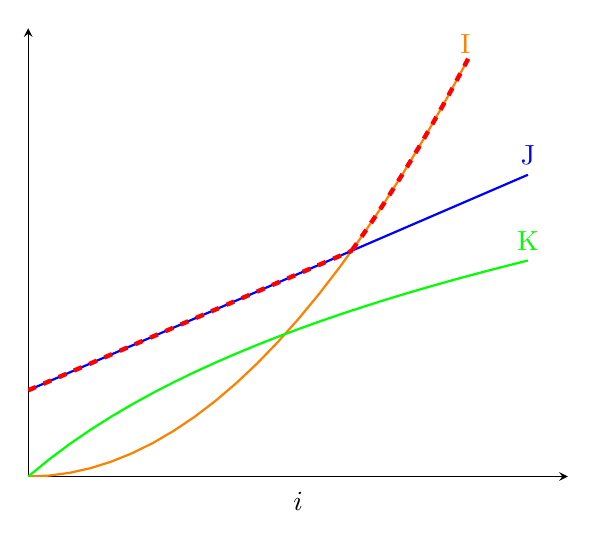
\begin{tikzpicture}
\begin{axis}[
    axis lines = left,
    xlabel = \(i\),
    ylabel = {},
    domain = 0:2.5,
    xtick={\empty},ytick={\empty},
    ymin=0,
    ymax=5.2,
    xmax=2.7,
    restrict y to domain=0:5,
]
    \addplot[thick, color=orange]{x^2} node[above,pos=1] {I};
    \addplot[thick, color=blue]{x+1} node[above,pos=1] {J};
    \addplot[thick, color=green]{ln(x+1)*2} node[above,pos=1] {K};
    \draw [ultra thick, dashed, draw=red] (axis cs:0,1) -- (axis cs:1.62,2.62);
    \addplot[ultra thick, color=green, dashed, color=red, domain=1.62:2.5]{x^2};
\end{axis}
\end{tikzpicture}
    \caption{Combined complexities illustrated. The combined complexity consists of the three indices I, J, K of the single index variable $i$. The dashed red line shows the bound of the combined complexity. $K$ is a superfluous index in the combined complexity as it never contributes to the bound of the combined complexity.}
    \label{fig:combined_complexity}
\end{figure}


\begin{defi}[Combined complexity]\label{def:combinedcomp} 
    We refer to a set $\kappa$ of complexities as a \textit{combined complexity}. We extend constraint judgements to include combined complexities such that
    \begin{enumerate}
        \item $\varphi;\Phi\vDash \kappa \leq \kappa'$ if for all $K \in \kappa$ there exists $K'\in \kappa'$ such that $\varphi;\Phi\vDash K \leq K'$.
        % 
        \item $\varphi;\Phi\vDash \kappa = \kappa'$ if $\varphi;\Phi\vDash \kappa \leq \kappa'$ and $\varphi;\Phi\vDash \kappa' \leq \kappa$.
        \item $\kappa + I = \{K + I \mid K \in \kappa\}$.
        %
        \item $\kappa\{J/i\} = \{ K\{J/i\} \mid K\in\kappa \}$.
    \end{enumerate}
    In the above, we may substitute an index for a combined complexity. In such judgements, the index represents a singleton set. For instance, $\varphi;\Phi\vDash \kappa \leq K$ represents $\varphi;\Phi\vDash \kappa \leq \{K\}$.
    %$\varphi;\Phi \vDash \kappa \bowtie \kappa' \quad\text{ if }\quad \forall K \in \kappa. (\exists K' \in \kappa'. \varphi;\Phi \vDash K \bowtie K')$.
\end{defi}

More specifically, when considering a combined complexity $\kappa$, we are interested in the maximal complexity given some valuation $\rho$, which we find by simply comparing the different values for the complexities within $\kappa$ given $\rho$. Note that the complexity $K \in \kappa$ that is maximal may be different for different valuations. In Definition \ref{def:combinedcomp} we extend the binary relations in $\bowtie$ on indices to combined complexities, such that we can compare two combined complexities such as $\varphi;\Phi \vDash \kappa \bowtie \kappa'$ and a combined complexity and complexity such as $\varphi;\Phi \vDash \kappa \bowtie K$. Definition \ref{def:combinedcompbasis} defines the function \textit{basis} that discards any $K \in \kappa$ that can never be the maximal complexity given some set of constraints $\Phi$ (i.e. the complexities that are bounded by other complexities in the set), such that we can always keep the number of complexities in a combined complexity to a minimum. %Finally, we may also be interested in adding an index onto a combined complexity, and so we define the addition of indices onto combined complexities in Definition \ref{def:combinedcompadd}.
%
\begin{defi}\label{def:combinedcompbasis}
    We define the function \textit{basis} that takes a set of index variables $\varphi$, a set of constraints $\Phi$ and a combined complexity $\kappa$, and returns a new combined complexity without superfluous complexities (The \textit{basis} of $\kappa$)
    \begin{align*}
        \text{basis}(\varphi,\Phi,\kappa) = \bigcap\left\{ \kappa' \subseteq \kappa \mid \forall K\in\kappa.\exists K'\in\kappa'.\varphi;\Phi\vDash K \leq K' \right\}
    \end{align*}
    Moreover, the algorithm below computes the basis
    % \begin{align*}
    %     \text{basis}(\varphi, \kappa) = \{(\Phi, K) \in \kappa \mid \varphi;\Phi \not \vDash K < K' \text{ for all } (\Phi', K') \in \kappa\}
    % \end{align*}
    \begin{align*}
        &\text{basis}(\varphi, \Phi, \kappa) = \text{do}\\[-0.5em]
        &\quad \kappa' \leftarrow \kappa\\[-0.5em]
        &\quad \text{for } K \in \kappa \text{ do}\\[-0.5em]
        &\quad\quad \text{ if } \exists K' \in \kappa' \text{ with } K \not = K' \text{ and } \varphi;\Phi \vDash K \leq K' \text{ then}\\[-0.5em]
        &\quad\quad\quad \kappa' \leftarrow \kappa' \setminus \{K\}\\[-0.5em]
        &\quad \text{return } \kappa'
    \end{align*}
\end{defi}
%
% \begin{defi}[]\label{def:combinedcompadd}
%     We define the the addition of a combined complexity and index as
%     \begin{align*}
%         \kappa + I = \{K + I \mid K \in \kappa\}
%     \end{align*}

% \end{defi}
%
For typing expressions, we use the rules presented in Table \ref{tab:sizedtypedexpressiontypes}, excluding the rule $\runa{BG-sub}$. In Table \ref{tab:sizedprocesstypingrules} we show the type rules for processes. Type judgements are of the form $\varphi;\Phi;\Gamma \vdash P \triangleleft \kappa$ where $\kappa$ denotes the complexity of process $P$. The rule $\runa{S-tick}$ types a \texttt{tick} prefix and incurs a cost of one in time complexity. We advance the time of all types in the context accordingly when typing the continuation. Rule $\runa{S-annot}$ is similar but may incur a cost of $n$. Matches on naturals are typed with rule $\runa{S-nmatch}$. Most notably, we extend the set of known constraints when typing the two continuations. That is, we can deduce constraints on the lower and upper bounds on the size of the expression we match on. For instance, for the zero pattern we can deduce that the lower bound $I$ must be equal to $0$ (or equivalently $I \leq 0$), and for the successor pattern, we can guarantee that the upper bound $J$ must be greater than or equal to $1$. For the complexity of pattern matches and parallel composition, we take advantage of the fact that we represent complexities using combined complexities. As such, we include complexities in both $P$ and $Q$ in the result. To remove redundancy from the set $\kappa \cup \kappa'$, we use the basis function.\\

%
% \begin{table*}[!ht]
%     \begin{framed}\vspace{-1em}\begin{align*}
%         &\kern15em\\[-2em] % Stretch frame
%         &\kern0em\runa{S-nil}\infrule{}{\varphi;\Phi;\Gamma \vdash \withcomplex{\nil}{0}} \kern1em\runa{S-tick}\;\infrule{\varphi;\Phi;\susumesim{\Gamma}{1}\vdash P \triangleleft K}{\varphi;\Phi;\Gamma\vdash \tick P \triangleleft K + 1} \kern3em\runa{S-nu}\;\infrule{\varphi;\Phi;\Gamma,\withtype{a}{T} \vdash \withcomplex{P}{K}}{\varphi;\Phi;\Gamma \vdash \newvar{a: T}{\withcomplex{P}{K}}}\\[-1em]
%         %
%         &\kern-0em\runa{S-nmatch}\;\condinfrule{
%         \begin{matrix}
%             \varphi;\Phi;\Gamma \vdash \withtype{e}{\natinterval{I}{J}}\quad \varphi;\Phi, I \leq 0;\Gamma \vdash \withcomplex{P}{K} \\
%             \varphi;\Phi, J \geq 1;\Gamma, \withtype{x}{\natinterval{I-1}{J-1}} \vdash \withcomplex{Q}{K'}
%         \end{matrix}}{\varphi;\Phi;\Gamma \vdash \withcomplex{\match{e}{P}{x}{Q}}{L}}{\text{where}\quad L = \left\{
% \begin{matrix}
%     K & \text{if}\; \varphi;\Phi\vDash K' \leq K   \\
%     K' & \text{if}\; \varphi;\Phi\vDash K \leq K'  \\
%     K+K' & \text{otherwise}
% \end{matrix}
% \right.}\\[-1em]
%         %
%         %&\kern-0em\runa{S-nmatch-2}\;\infrule{
%         %\begin{matrix}
%         %    \varphi;\Phi;\Gamma \vdash \withtype{e}{\natinterval{I}{J}} \quad \varphi;\Phi\vDash K \leq K' \\
%         %    \varphi;\Phi, I \leq 0;\Gamma \vdash \withcomplex{P}{K} \quad \varphi;\Phi, J \geq 1;\Gamma, \withtype{x}{\natinterval{I-1}{J-1}} \vdash \withcomplex{Q}{K'}
%         %\end{matrix}}{\varphi;\Phi;\Gamma \vdash \withcomplex{\match{e}{P}{x}{Q}}{K'}}\\[-1em]
%         %
%         &\kern-0em\runa{S-lmatch}\;\condinfrule{
%         \begin{matrix}
%             \varphi;\Phi;\Gamma \vdash \withtype{e}{\texttt{List}[I,J](\mathcal{B})} \quad \varphi;\Phi, I \leq 0;\Gamma \vdash \withcomplex{P}{K} \\
%             \varphi;\Phi, J \geq 1;\Gamma, \withtype{x}{\mathcal{B}},y : \texttt{List}[I-1,J-1](\mathcal{B}) \vdash \withcomplex{Q}{K'}
%         \end{matrix}}{\varphi;\Phi;\Gamma \vdash \withcomplex{\texttt{match}\;e\;\{ [] \mapsto P;\; x :: y \mapsto Q \}}{L}}{\text{where}\quad L = \left\{
% \begin{matrix}
%     K & \text{if}\; \varphi;\Phi\vDash K' \leq K   \\
%     K' & \text{if}\; \varphi;\Phi\vDash K \leq K'  \\
%     K+K' & \text{otherwise}
% \end{matrix}
% \right.}\\[-1em]
%         %
%         %&\kern-0em\runa{S-lmatch-2}\;\infrule{
%         %\begin{matrix}
%         %    \varphi;\Phi;\Gamma \vdash \withtype{e}{\texttt{List}[I,J](\mathcal{B})} \quad \varphi;\Phi\vDash K \leq K' \\
%         %    \varphi;\Phi, I \leq 0;\Gamma \vdash \withcomplex{P}{K} \quad \varphi;\Phi, J \geq 1;\Gamma, \withtype{x}{\mathcal{B}},y : \texttt{List}[I-1,J-1](\mathcal{B}) \vdash \withcomplex{Q}{K'}
%       % \end{matrix}}{\varphi;\Phi;\Gamma \vdash \withcomplex{\texttt{match}\;e\;\{ [] \mapsto P;\; x :: y \mapsto Q \}}{K'}}\\[-1em]
%         %
%         &\kern4em\runa{S-par}\;\condinfrule{\varphi;\Phi;\Gamma\vdash P \triangleleft K\quad \varphi;\Phi;\Gamma\vdash Q \triangleleft K'}{\varphi;\Phi;\Gamma\vdash \parcomp{P}{Q} \triangleleft L}{\text{where}\quad L = \left\{
% \begin{matrix}
%     K & \text{if}\; \varphi;\Phi\vDash K' \leq K   \\
%     K' & \text{if}\; \varphi;\Phi\vDash K \leq K'  %\\
%     %K+K' & \text{otherwise}
% \end{matrix}
% \right.}\\[-1em]
%         %
%         %&\kern4em\runa{S-par-2}\;\infrule{\varphi;\Phi;\Gamma\vdash P \triangleleft K\quad \varphi;\Phi;\Gamma\vdash Q \triangleleft K'\quad \varphi;\Phi\vDash K \leq K'}{\varphi;\Phi;\Gamma\vdash \parcomp{P}{Q} \triangleleft K'}\\[-1em]
%         %
%         &\kern-0em\runa{S-iserv}\;\infrule{\texttt{in}\in\sigma\quad \varphi,\widetilde{i};\Phi;\text{ready}(\varphi,\Phi,\susumesim{\Gamma}{I}),a:\forall_0\widetilde{i}.\texttt{serv}^{\sigma\cap\{\texttt{out}\}}_K(\widetilde{T}),\widetilde{v} : \widetilde{T}\vdash P \triangleleft K'\quad \varphi,\widetilde{i};\Phi\vDash K' \leq K}{\varphi;\Phi;\Gamma,a:\forall_I\widetilde{i}.\texttt{serv}^\sigma_K(\widetilde{T})\vdash\; \bang\inputch{a}{\widetilde{v}}{}{P}\triangleleft I}\\[-1em]
%         %
%         &\kern-0em\runa{S-ich}\;\infrule{\texttt{in}\in\sigma\quad \varphi;\Phi;\susumesim{\Gamma}{I},a:\texttt{ch}_0^\sigma(\widetilde{T}),\widetilde{v} : \widetilde{T}\vdash P \triangleleft K}{\varphi;\Phi;\Gamma,a:\texttt{ch}_I^\sigma(\widetilde{T})\vdash \inputch{a}{\widetilde{v}}{}{P}\triangleleft K + I}
%         %
%         \kern8.5em \runa{S-och}\;\infrule{\texttt{out}\in \sigma\quad \varphi;\Phi;\susumesim{\Gamma}{I}\vdash \widetilde{e} : \widetilde{T}\quad \varphi;\Phi\vdash\widetilde{T}\sqsubseteq\widetilde{S}}{\varphi;\Phi;\Gamma,a:\texttt{ch}^{\sigma}_I(\widetilde{S})\vdash \asyncoutputch{a}{\widetilde{e}}{} \triangleleft I}\\[-1em]
%         %
%         &\kern0em\runa{S-oserv}\;\infrule{\texttt{out} \in \sigma \quad \varphi;\Phi;\susumesim{\Gamma}{I}\vdash \widetilde{e} : \widetilde{T}\quad \text{instantiate}(\widetilde{i},\widetilde{T})=\{\widetilde{J}/\widetilde{i}\}\quad  \varphi;\Phi\vdash\widetilde{T}\sqsubseteq\widetilde{S}\{\widetilde{J}/\widetilde{i}\}}{\varphi;\Phi;\Gamma,a:\forall_I\widetilde{i}.\texttt{serv}_K^\sigma(\widetilde{S})\vdash \asyncoutputch{a}{\widetilde{e}}{} \triangleleft K\!\substi{\widetilde{J}}{\widetilde{i}} + I}
%         %
%     \end{align*}\vspace{-1em}\end{framed}
%     \smallskip
%     \caption{Sized typing rules for parallel complexity of processes.}
%     \label{tab:sizedprocesstypingrules}
% \end{table*}

\begin{table*}[!ht]
    \begin{framed}\vspace{-1em}\begin{align*}
        %
        % S-nil
        &\runa{S-nu}\infrule{\varphi;\Phi;\Gamma, a:T \vdash P \triangleleft \kappa}{\varphi;\Phi;\Gamma \vdash \newvar{a:T}{P} \triangleleft \kappa}
        % S-par
        \kern1em\runa{S-par}\infrule{\varphi;\Phi;\Gamma \vdash P \triangleleft \kappa \quad \varphi;\Phi;\Gamma \vdash Q \triangleleft \kappa'}{\varphi;\Phi;\Gamma \vdash P \mid Q \triangleleft \text{basis}(\varphi, \Phi,\kappa \cup \kappa')}\\[-1em]
        %
        &\runa{S-tick}\infrule{\varphi;\Phi;\tforwardsim{\Gamma}{1} \vdash P \triangleleft \kappa}{\varphi;\Phi;\Gamma \vdash \tick P \triangleleft \kappa + 1}\kern2em
        %
        \runa{S-annot}\infrule{\varphi;\Phi;\tforwardsim{\Gamma}{n}\vdash P \triangleleft \kappa}{\varphi;\Phi;\Gamma\vdash n:P \triangleleft \kappa + n}\\[-1em]
        % S-match
        &\runa{S-match}\infrule{
        \begin{matrix}
            \varphi;\Phi;\Gamma \vdash e:\natinterval{I}{J} \quad \varphi;\Phi, I \leq 0;\Gamma \vdash P \triangleleft \kappa\\
            \varphi;\Phi, J \geq 1;\Gamma, x:\natinterval{I-1}{J-1} \vdash Q \triangleleft \kappa'
        \end{matrix}}{\varphi;\Phi;\Gamma \vdash \match{e}{P}{x}{Q} \triangleleft \text{basis}(\varphi, \Phi, \kappa \cup \kappa')}\\[-1em]
        % S-iserv
        &\runa{S-iserv}\infrule{\begin{matrix}
            \texttt{in} \in \sigma\quad \varphi;\Phi;\Gamma\vdash a:\servt{I}{i}{\sigma}{K}{\widetilde{T}}\\
            \varphi, \widetilde{i}; \Phi; \text{ready}(\varphi,\Phi,\tforwardsim{\Gamma}{I}), \widetilde{v} : \widetilde{T} \vdash P \triangleleft \kappa \quad \varphi,\widetilde{i};\Phi\vDash\kappa \leq K
        \end{matrix}}
        {\varphi;\Phi;\Gamma \vdash \;\bang\inputch{a}{\widetilde{v}}{}{P}\triangleleft \{I\}}
        %
        \kern14em\runa{S-nil}\kern-1em\infrule{}{\varphi;\Phi;\Gamma \vdash \nil \triangleleft \{0\}}\kern-3em\text{ }\\[-1em]
        % S-oserv
        &\runa{S-oserv}\infrule{\begin{matrix}
            \texttt{out} \in \sigma\quad \varphi;\Phi;\Gamma\vdash a:\servt{I}{i}{\sigma}{K}{\widetilde{T}}\\
            \varphi; \Phi;\tforwardsim{\Gamma}{I} \vdash \widetilde{e}:\widetilde{S} \quad \text{instantiate}(\widetilde{i}, \widetilde{S}) = \{\widetilde{J}/\widetilde{i}\} \quad \varphi;\Phi \vDash \widetilde{S} \sqsubseteq \widetilde{T}
        \end{matrix}}
        {\varphi;\Phi;\Gamma \vdash \asyncoutputch{a}{\widetilde{e}}{}\triangleleft \{K\{\widetilde{J}/\widetilde{i}\} + I\}}\\[-1em]
        % S-annot
        &\runa{S-ich}\infrule{\begin{matrix}
            \texttt{in} \in \sigma\quad \varphi;\Phi;\Gamma \vdash a:\chant{\sigma}{I}{\widetilde{T}}\\
            \varphi; \Phi; \tforwardsim{\Gamma}{I}, \widetilde{v}:\widetilde{T} \vdash P \triangleleft \kappa
        \end{matrix}}
        {\varphi;\Phi;\Gamma \vdash \inputch{a}{\widetilde{v}}{}{P} \triangleleft \kappa + I}\kern3em
        %
        \runa{S-och}\infrule{\begin{matrix}
            \texttt{out} \in \sigma\quad \varphi;\Phi;\Gamma \vdash a:\chant{\sigma}{I}{\widetilde{T}}\\
            \varphi; \Phi; \tforwardsim{\Gamma}{I} \vdash \widetilde{e}:\widetilde{S} \quad \varphi;\Phi \vDash \widetilde{S} \sqsubseteq \widetilde{T}
        \end{matrix}}
        {\varphi;\Phi;\Gamma \vdash \asyncoutputch{a}{\widetilde{e}}{} \triangleleft \{I\}}\\[-1em]
    \end{align*}\vspace{-1em}\end{framed}
    \smallskip
    \caption{Sized typing rules for parallel complexity of processes.}
    \label{tab:sizedprocesstypingrules}
\end{table*}

%
Rule $\runa{S-iserv}$ types a replicated input on a name $a$, and so $a$ must be bound to a server type with input capability. As the index $I$ in the server type denotes the time steps remaining before the server is ready to synchronize, we advance the time by $I$ units of time complexity when typing the continuation $P$. To ensure that bounds on synchronizations in $\downarrow^{\varphi;\Phi}_I\!\Gamma$ are not violated, we type $P$ under the time invariant part of $\downarrow^{\varphi;\Phi}_I\!\Gamma$, i.e. $\text{ready}(\varphi,\Phi,\downarrow_I\!\Gamma)$. Note that the bound on the span of the replicated input is the bound on the time remaining before the server is ready to synchronize. As the replicated input may be invoked many times, the cost of invoking the server is accounted for in rule $\runa{S-oserv}$ using the complexity bound $K$ in the server type. Therefore, we enforce that $K$ is in fact an upper bound on the span of the continuation $P$.\\

The rule $\runa{S-oserv}$ types outputs on names bound to server types. Here, as stated above, we must account for the cost of invoking a server, and as a replicated input on a server is parametric, we must \textit{instantiate} it based on the types of the expressions we are to output. Recall that in the type rule for outputs on servers from Chapter \ref{ch:bgts}, this is to be done by finding a substitution that satisfies the premise $\widetilde{T} \sqsubseteq \widetilde{S}\{\widetilde{J}/\widetilde{i}\}$. However, this turns out to be a difficult problem, and we can in fact prove it NP-complete for types of polynomial indices even if we disregard subtyping. However, note that it might not be necessary to use the full expressive power of polynomial indices, and so this may not necessarily affect type checking. Nevertheless, we over-approximate finding such a substitution, by using the function $\textit{instantiate}$. That is, we \textit{zip} together the index variables $\widetilde{i}$ with indices in types $\widetilde{T}$. Remark that Baillot and Ghyselen \cite{BaillotGhyselen2021} propose types for inference in their technical report, where the problem is simplified substantially, by forcing naturals to have lower bounds of $0$ and upper bounds with exactly one index variable and a constant. Our approach admits more expressive lower bounds and multiplications, while imposing no direct restrictions on the number of index variables in an index, and is thus more suitable for a type-checker.\\

We now prove the NP-completeness of the smaller problem of checking whether there exists a substitution $\{\widetilde{J}/\widetilde{i}\}$ that satisfies $T = S\{\widetilde{J}/\widetilde{i}\}$ where $T$ and $S$ are types with polynomial indices. The main idea is a reduction proof from the NP-complete 3-SAT problem, i.e. the satisfiability problem of a boolean formula in conjunctive normal form with exactly three literals in each clause \cite{Karp1972}. We first define a translation from a 3-SAT formula to a polynomial index in Definition \ref{def:3satredu}. This is a polynomial time computable reduction, as we simply replace each logical-and with a multiplication, each logical-or with an addition and each negation with a subtraction from 1. In Lemma \ref{lemma:soundtranslation}, we prove that the reduction is faithful with respect to satisfiability of a boolean formula. Finally, in Lemma \ref{lemma:npcompletesubst}, we prove that it is an NP-complete decision problem to verify the existence of a substitution that satisfies $T = S\{\widetilde{J}/\widetilde{i}\}$ for types $T$ and $S$.
%
\begin{defi}[3-SAT reduction]\label{def:3satredu}
We assume a one-to-one mapping $f$ from unknowns to index variables. Let $\phi$ be a 3-SAT formula
\begin{align*}
    \phi = \bigwedge_{i=1}^n \left(\ell_{i1} \lor \ell_{i2} \lor \ell_{i3}\right)% \land \cdots \land (A_n \lor B_n \lor C_n)
\end{align*}
where $\ell_{i1}$, $\ell_{i2}$ and $\ell_{i3}$ are of the forms $x$ or $\neg x$ for some variable $x$. We define a translation of $\phi$ to a polynomial index %$[\![\phi]\!]_{\text{3-SAT}}$
\begin{align*}
    [\![\phi]\!]_{\text{3-SAT}} = \prod_{i=1}^n \left([\![\ell_{i1}]\!]_{\text{3-SAT}} + [\![\ell_{i2}]\!]_{\text{3-SAT}} + [\![\ell_{i3}]\!]_{\text{3-SAT}}\right) %\cdots ([\![A_n]\!]_{\text{3-SAT}} + [\![B_n]\!]_{\text{3-SAT}} + [\![C_n]\!]_{\text{3-SAT}})
\end{align*}
where $[\![x]\!]_{\text{3-SAT}} = f(x)$ and $[\![\neg x]\!]_{\text{3-SAT}} = (1 - f(x))$.
\end{defi}


\begin{lemma}\label{lemma:soundtranslation}
Let $\phi$ be a 3-SAT formula. Then $\phi$ is satisfiable if and only if there exists a substitution $\{\widetilde{n}/\widetilde{i}\}$ such that $1\leq [\![\phi]\!]_{\text{3-SAT}}\{\widetilde{n}/\widetilde{i}\}$.
\begin{proof}
We consider the implications separately
\begin{enumerate}
    \item Assume that $\phi$ is satisfiable. Then there exists a truth assignment $\tau$ such that each clause of $\phi$ is true. Correspondingly, as $[\![\phi]\!]_{\text{3-SAT}}$ is a product of non-negative factors, we for some substitution $\{\widetilde{n}/\widetilde{i}\}$ have that $1 \leq [\![\phi]\!]_{\text{3-SAT}}\{\widetilde{n}/\widetilde{i}\}$ if and only if each factor in the product is positive. We compare the conditions for a clause to be true in $\phi$ to those for a corresponding factor in $[\![\phi]\!]_{\text{3-SAT}}$ to be positive, and show that a substitution $\{\widetilde{n}/\widetilde{i}\}$ exists such that $1 \leq [\![\phi]\!]_{\text{3-SAT}}\{\widetilde{n}/\widetilde{i}\}$. A clause in $\phi$ is a disjunction of three literals of either the form $x$ or $\neg x$ for some unknown $x$. Thus, for a clause to be true, we must have at least one literal $\tau(x) = tt$ or $\neg \tau(x) = tt$ with $\tau(x) = f\!f$. The corresponding factor in $[\![\phi]\!]_{\text{3-SAT}}$ is a sum of three terms of the forms $f(x)$ or $(1 - f(x))$ for some unknown $x$, where $f$ is a one-to-one mapping from unknowns to index variables. Here, we utilize that in the type system by Baillot and Ghyselen \cite{BaillotGhyselen2021}, we have $(1 - i\{\widetilde{n}/\widetilde{i}\}) = 0$ when $i\{\widetilde{n}/\widetilde{i}\} \geq 1$ and $(1 - i\{\widetilde{n}/\widetilde{i}\}) = 1$ when $i\{\widetilde{n}/\widetilde{i}\} = 0$. Thus, for a factor to be positive, it suffices that one term is positive, and so we can construct a substitution that guarantees this from the interpretation of $\phi$. That is, if $\tau(x) = tt$, we substitute $1$ for $f(x)$, and if $\tau(x) = f\!f$, we substitute 0 for $f(x)$. Then, whenever a literal is true in $\phi$, the corresponding term in $[\![\phi]\!]_{\text{3-SAT}}$ is positive, and so if $\phi$ is satisfiable then there exists a substitution $\{\widetilde{n}/\widetilde{i}\}$ such that $1 \leq [\![\phi]\!]_{\text{3-SAT}}\{\widetilde{n}/\widetilde{i}\}$.
     
    \item Assume that there exists a substitution $\{\widetilde{n}/\widetilde{i}\}$ such that $1 \leq [\![\phi]\!]_{\text{3-SAT}}\{\widetilde{n}/\widetilde{i}\}$. Then, as $[\![\phi]\!]_{\text{3-SAT}}$ is a product of non-negative factors, each factor must be positive. Correspondingly, if $\Phi$ is satisfiable, then there exists a truth assignment such that each clause of $\phi$ is true. We compare the conditions for a factor in $[\![\phi]\!]_{\text{3-SAT}}\{\widetilde{n}/\widetilde{i}\}$ to be positive to those for a corresponding clause in $\phi$ to be true, and show that $\phi$ is satisfiable. A factor in $[\![\phi]\!]_{\text{3-SAT}}$ is a sum of at most three terms of the forms $f(x)\{\widetilde{n}/\widetilde{i}\}$ or $(1 - f(x)\{\widetilde{n}/\widetilde{i}\})$. Here we again utilize that in the type system by Baillot and Ghyselen \cite{BaillotGhyselen2021}, we have $(1 - f(x)\{\widetilde{n}/\widetilde{i}\}) = 0$ when $f(x)\{\widetilde{n}/\widetilde{i}\} \geq 1$ and $(1 - f(x)\{\widetilde{n}/\widetilde{i}\}) = 1$ when $f(x)\{\widetilde{n}/\widetilde{i}\} = 0$, and so it must be that in the factor, we have at least one term $f(x)\{\widetilde{n}/\widetilde{i}\} \geq 1$ or $(1 - f(x)\{\widetilde{n}/\widetilde{i}\}) \geq 1$. Correspondingly, for the clause in $\phi$ to be true, at least one literal must be true. We show that there exists a truth assignment $\tau$ such that if a term in $[\![\phi]\!]_{\text{3-SAT}}$ is positive, then the corresponding literal in $\phi$ is true. If $f(x)\{\widetilde{n}/\widetilde{i}\}\geq 1$ then we set $\tau(x) = tt$, and if $f(x)\{\widetilde{n}/\widetilde{i}\} = 0$ we set $\tau(x) = f\!f$, as $[\![x]\!]_{\text{3-SAT}}\{\widetilde{n}/\widetilde{i}\} \geq 1$ when $f(x)\{\widetilde{n}/\widetilde{i}\} \geq 1$ and $[\![\neg x]\!]_{\text{3-SAT}} \geq 1$ when $f(x)\{\widetilde{n}/\widetilde{i}\}=0$. Then, whenever a term is positive in $[\![\phi]\!]_{\text{3-SAT}}\{\widetilde{n}/\widetilde{i}\}$, the corresponding literal in $\phi$ is true, and so if there exists a substitution $\{\widetilde{n}/\widetilde{i}\}$ such that $1 \leq [\![\phi]\!]_{\text{3-SAT}}\{\widetilde{n}/\widetilde{i}\}$, then $\phi$ is satisfiable.
    
\end{enumerate}
\end{proof}
\end{lemma}


\begin{lemma}\label{lemma:npcompletesubst}
Let $T$ and $S$ be types with polynomial indices. Then checking whether there exists a substitution $\{\widetilde{J}/\widetilde{i}\}$ such that $T = S\{\widetilde{J}/\widetilde{i}\}$ is an NP-complete problem.
\begin{proof}
By reduction from the 3-SAT problem. Assume that we have some algorithm that can verify the existence of a substitution $\{\widetilde{J}/\widetilde{i}\}$ such that $T = S\{\widetilde{J}/\widetilde{i}\}$, and let $\phi$ be a 3-SAT formula. Then using the algorithm, we can check whether $\phi$ is satisfiable by verifying whether there exists $\{\widetilde{J}/\widetilde{i}\}$ such that the following holds
\begin{align*}
    \texttt{Nat}[0,1] = \texttt{Nat}[0,(1 - (1 - [\![\phi]\!]_{\text{3-SAT}}))]\{\widetilde{J}/\widetilde{i}\}
\end{align*}
That is, $1 = (1 - (1 - [\![\phi]\!]_{\text{3-SAT}}\{\widetilde{J}/\widetilde{i}\}))$ implies $1 \leq [\![\phi]\!]_{\text{3-SAT}}\{\widetilde{J}/\widetilde{i}\}$, as $(1 - [\![\phi]\!]_{\text{3-SAT}}\{\widetilde{J}/\widetilde{i}\}) = 0$ when $[\![\phi]\!]_{\text{3-SAT}}\{\widetilde{J}/\widetilde{i}\} \geq 1$ and $(1 - [\![\phi]\!]_{\text{3-SAT}}\{\widetilde{J}/\widetilde{i}\}) = 1$ when $[\![\phi]\!]_{\text{3-SAT}}\{\widetilde{J}/\widetilde{i}\} = 0$. Furthermore, for $1 \leq [\![\phi]\!]_{\text{3-SAT}}\{\widetilde{J}/\widetilde{i}\}$ to hold, the indices in the sequence $\widetilde{J}$ cannot contain index variables, and so there must exist an equivalent substitution of naturals for index variables $\{\widetilde{n}/\widetilde{i}\}$. Then, by Lemma \ref{lemma:soundtranslation} we have that $\phi$ is satisfiable if and only if there exists a substitution $\{\widetilde{n}/\widetilde{i}\}$ such that $1\leq [\![\phi]\!]_{\text{3-SAT}}\{\widetilde{n}/\widetilde{i}\}$. Thus, as 3-SAT is an NP-complete problem, the reduction from 3-SAT is computable in polynomial time and as polynomial reduction is a transitive relation, i.e. any NP-problem is polynomial time reducible to verifying the existence of a substitution $\{\widetilde{J}/\widetilde{i}\}$ that satisfies the equation $T = S\{\widetilde{J}/\widetilde{i}\}$, it follows that the problem is NP-hard. To show that it is an NP-complete problem, we show that a \textit{certificate} can be verified in polynomial time. That is, given some substitution $\{\widetilde{J}/\widetilde{i}\}$, we can in linear time check whether $T=S\{\widetilde{J}/\widetilde{i}\}$ by substituting indices $\widetilde{J}$ for indices $\widetilde{i}$ in type $S$ and by then comparing the two types.\\
%
%
%Utilizing that $n - m = 0$ for $m\geq n$ in the type system of Baillot and Ghyselen \cite{BaillotGhyselen2021}, we can simulate any boolean formula using a polynomial index. By denoting $J = 0$ false and $I > 0$ true, we have the translation
% \begin{align*}
%     [\![a \land b]\!]_\phi =&\; [\![a]\!]_\phi [\![b]\!]_\phi\\
%     [\![a \lor b]\!]_\phi =&\; [\![a]\!]_\phi + [\![b]\!]_\phi\\
%     [\![\neg a]\!]_\phi =&\; (1 - [\![a]\!]_\phi)\\
%     [\![x]\!]_\phi =&\; i
% \end{align*}
% Then assuming some algorithm that checks whether there exists a substitution $\{\widetilde{J}/\widetilde{i}\}$ such that $T \sqsubseteq S\{\widetilde{J}/\widetilde{i}\}$, we can solve the boolean satisfiability problem. Let $\phi_0$ be any boolean formula and let $\widetilde{i}$ be the index variables in $[\![\phi_0]\!]_\phi$, and assume that there exists a substitution $\{\widetilde{J}/\widetilde{i}\}$ that satisfies the judgement
% \begin{align*}
%     \emptyset;\emptyset\vDash\texttt{Nat}[0,1] \sqsubseteq \texttt{Nat}[0,[\![\phi_0]\!]_\phi]\{\widetilde{J}/\widetilde{i}\}
% \end{align*}
% Then by rule $\runa{SS-nweak}$ we have that $\emptyset;\emptyset\vDash 1 \leq [\![\phi_0]\!]_\phi\{\widetilde{J}/\widetilde{i}\}$, and as $\varphi = \emptyset$, the indices $\widetilde{J}$ must be constants. Thus, $\emptyset;\emptyset\vDash 1 \leq [\![\phi_0]\!]_\phi\{\widetilde{J}/\widetilde{i}\}$ is equivalent to $1 \leq [\![\phi_0]\!]_\phi\{\widetilde{J}/\widetilde{i}\}$, and so $\phi_0$ must have a solution. If instead no such substitution exists, then for any $\{\widetilde{J}/\widetilde{i}\}$, it must be that $[\![\phi_0]\!]_\phi\{\widetilde{J}/\widetilde{i}\} = 0$ implying that $\phi_0$ is a contradiction. Therefore, as the boolean satisfiability problem is NP-complete, the algorithm we assumed must be NP-complete as well.
\end{proof}
\end{lemma}

In Example \ref{example:addition}, we show how a process implementing addition of naturals can be typed using our type rules, yielding a precise bound on the parallel complexity.
%

\begin{examp}\label{example:addition}
As an example of a process that is typable using our type rules, we show how the addition operator for naturals can be written as a process and subsequently be typed. We use a server to encode the addition operator
\begin{align*}
    !\inputch{\text{add}}{x,y,r}{}{\match{x}{\asyncoutputch{r}{y}{}}{z}{\tick{\asyncoutputch{\text{add}}{z,\succc y,r}{}}}}
\end{align*}
such that channel $r$ is used to output the addition of naturals $x$ and $y$. To type the process, we use the following contexts and set of index variables
\begin{align*}
    \Gamma\defeq&\; \text{add} : \forall_0 i,j,k,l,m,n,o.\texttt{serv}^{\{\texttt{in},\texttt{out}\}}_j(\texttt{Nat}[0,j],\texttt{Nat}[0,l],\texttt{ch}^{\{\texttt{out}\}}_j(\texttt{Nat}[0,j+l])) \\
    \Delta\defeq&\; \text{ready}(\cdot,\cdot,\Gamma), x : \texttt{Nat}[0,j], y: \texttt{Nat}[0,l], r:\texttt{ch}^{\{\texttt{out}\}}_j(\texttt{Nat}[0,j+l])\\
    \varphi \defeq&\; \{i,j,k,l,m,n,o\}
\end{align*}
%
We now derive a type for the encoding of the addition operator, yielding a precise bound of $j$, corresponding to an upper bound on the size of $x$, as we pattern match at most $j$ times on natural $x$. Notably we have that $\text{instantiate}((i,j,k,l,m,n,o),\texttt{Nat}[0,j\monus 1],\texttt{Nat}[1,l+1],\texttt{ch}^{\{\texttt{out}\}}_j(\texttt{Nat}[0,j+l]))=\{0/i,j\monus 1/j,0/k,l+1/l,j/m,0/n,j+l/o\}$.
%
{\small
\begin{align*}
    \begin{prooftree}
        %
        \infer0{\varphi;\cdot,0\leq 0;\Delta\vdash \asyncoutputch{r}{y}{} \triangleleft \{j\}}
        %
        % \infer0{\texttt{Nat}[0,j\monus 1] \sqsubseteq \texttt{Nat}[0,j]\{j\monus 1/j\}}
        % %
        % \infer0{\texttt{Nat}[0,l+1] \sqsubseteq \texttt{Nat}[0,l]\{l+1/l\}}
        % %
        % \infer0{\texttt{ch}^{\{\texttt{out}\}}_{j\monus 1}(\texttt{Nat}[0,j+l] \sqsubseteq \texttt{ch}^{\{\texttt{out}\}}_{j\monus 1}(\texttt{Nat}[0,j+l)\{j\monus 1/j,l+1/l\}}
        %
        \infer0{
        \begin{matrix}
        \varphi;\cdot,1\leq j\vdash\texttt{Nat}[0,j\monus 1] \sqsubseteq \texttt{Nat}[0,j]\{j\monus 1/j\}\\
        \varphi;\cdot,1\leq j\vdash\texttt{Nat}[1,l+1] \sqsubseteq \texttt{Nat}[0,l]\{l+1/l\}\\
        \varphi;\cdot,1\leq j\vdash\texttt{ch}^{\{\texttt{out}\}}_{j\monus 1}(\texttt{Nat}[0,j+l] \sqsubseteq \texttt{ch}^{\{\texttt{out}\}}_{j\monus 1}(\texttt{Nat}[0,j+l)\{j\monus 1/j,l+1/l\}
        \end{matrix}
        }
        %
        \infer1{\varphi;\cdot,1\leq j;\susumesim{\Delta}{1},z : \texttt{Nat}[0,j\monus 1]\vdash \asyncoutputch{\text{add}}{z,\succc y, r}{} \triangleleft \{j\monus 1\}}
        %
        \infer1{\varphi;\cdot,1\leq j;\Delta,z : \texttt{Nat}[0,j\monus 1]\vdash \tick{\asyncoutputch{\text{add}}{z,\succc y, r}{}} \triangleleft \{j\}}
        %
        \infer2{\varphi;\cdot;\Delta\vdash \match{x}{\asyncoutputch{r}{y}{}}{z}{\tick{\asyncoutputch{\text{add}}{z,\succc y,r}{}}} \triangleleft \{j\}}
        %
        \infer1{\cdot;\cdot;\Gamma\vdash\; !\inputch{\text{add}}{x,y,r}{}{\match{x}{\asyncoutputch{r}{y}{}}{z}{\tick{\asyncoutputch{\text{add}}{z,\succc y,r}{}}}}\triangleleft \{0\}}
    \end{prooftree}
\end{align*}}
%
\end{examp}

% \subsection{Undecidability of judgements}
% Verifying whether a polynomial constraint with integer coefficients imposes further restrictions onto the model set of index valuations of natural codomain of some set of known constraints can be reduced to Hilbert's tenth problem \cite{Davis1973}. That is, the problem of verifying whether a diophantine equation has an integer solution.\\

% We first assume some algorithm that can verify a judgement of the form $\varphi;\Phi\vDash C$ where $\varphi$ is a set of index variables and $C$ and $C'\in\Phi$ are binary constraints on polynomials of integer coefficients over relations from any subset of $\{\neq,\leq, <\}$. Recall that such a judgement holds exactly when for each index valuation $\rho : \varphi \longrightarrow \mathbb{N}$ over $\varphi$ for which $\rho \vDash C'$ for $C'\in\Phi$ we also have $\rho\vDash C$, i.e. $C$ does not impose further restrictions on interpretations of indices.\\

% We can then verify whether any diophantine equation has an integer solution. Let $p$ be an arbitrary polynomial of integer coefficients such that $p = 0$ is a diophantine equation. As only non-negative integers substitute for index variables, we first transform $p = 0$ to a new diophantine equation $p' = 0$ that has a non-negative integer solution exactly when $p = 0$ has an integer solution. To do this, we simply replace each index variable $i$ in $p$ with two new index variables $i_1 - i_2$. Then the judgement $\varphi;\emptyset\vDash p' \neq 0$ holds exactly when $p=0$ has no integer solution. That is, if $p=0$ has an integer solution, then there must exist a valuation $\rho_0$ such that $\rho_0\vDash \emptyset$ with $[\![p']\!]_{\rho_0} = 0$ and so $\rho_0\nvDash p' \neq 0$. Moreover, we need not rely on the relation $\neq$, as the judgements below are equivalent
% \begin{align*}
%     \varphi;\{p' \leq 0\} \vDash p' < 0\\
%     \varphi;\{p' \leq 0\} \vDash p' \leq 1
% \end{align*}
\section{Soundness}
\section{Verification of constraint judgements}\label{sec:verifyinglinearjudgements}
Until now we have not considered how we can verify constraint judgements in the type rules. The expressiveness of implementations of the type system by Baillot and Ghyselen \cite{BaillotGhyselen2021} depends on both the expressiveness of indices and whether judgements on the corresponding constraints are decidable. Naturally, we are interested in both of these properties, and so in this section, we show how judgements on linear constraints can be verified using algorithms. Later, we show how this can be extended to certain groups of polynomial constraints. We first make some needed changes to how the type checker uses subtraction.
%
\subsection{Subtraction of naturals}
The constraint judgements rely on a special minus operator ($\monus$) for indices such that $n \monus m=0$ when $m \geq n$, which we refer to as the \textit{monus} operator. This is apparent in the pattern match constructor type rule from Chapter \ref{ch:bgts}. Without this behavior, we may encounter problems when checking subtype premises in match processes. This has the consequence that equations such as $2\monus 3+3=3$ hold, such that indices form a semiring rather than a ring, as we are no longer guaranteed an additive inverse. In general, semirings lack many properties of rings that are desirable. For example, given two seemingly equivalent constraints $i \leq 5$ and $i \monus 5 \leq 0$, we see that by adding any constant to their left-hand sides, the constraints are no longer equivalent. Adding the constant 2 to their left-hand sides, we obtain $i + 2 \leq 5$ and $i \monus 5 + 2 \leq 0$, however, we see that the first constraint is satisfied given the valuation $i = 3$ but the second is not. In general the associative property of $+$ is lost.\\

Unfortunately, this is not an easy problem to solve implementation-wise, as indices are not actually evaluated but rather represent whole feasible regions. Thus, instead of trying to implement this operator exactly, we limit the number of processes typable by the type system. Removing the operator entirely is not an option as it us used by the type rules themselves. Instead, we ensure that one cannot \textit{exploit} the special behavior of monus by introducing additional conditions to the type rules of the type system. More precisely, any time the type system uses the monus operator such as $I \monus J$, we require the premise $\varphi;\Phi \vDash I \geq J$, in which case the monus operator is safe to treat as a regular minus. This, however, puts severe restrictions on the number of processes typable, and so we relax the restriction a bit by also checking the judgement $\varphi;\Phi \vDash I \leq J$, in which case we can conclude that the result is definitely $0$. If neither $\varphi;\Phi\vDash I \geq J$ nor $\varphi;\Phi\vDash I \leq 0$ hold, which is possible as $\leq$ and $\geq$ do not form a total order on indices, the result is undefined. We refer to this variant of monus as the \textit{partial} monus operator, as formalized in Definition \ref{def:partialmonus}. Note that this definition of monus allows us to obtain identical behavior to minus on a constraint $I \bowtie J$ by moving terms between the LHS and RHS, i.e. $I - K \bowtie J \Rightarrow I \bowtie J + K$, and so we can assume we have a standard minus operator when verifying judgements on constraints. For the remainder of this section, we assume this definition is used in the type rules instead of the usual monus. We may omit $\varphi;\Phi$ if it is clear from the context.%\\
%
%Definition \ref{def:partialmonus} defines the \textit{partial} monus operator that is undefined if we cannot determine if the result is either always positive or always zero. For the remainder of this thesis, we assume this definition is used in the type rules instead of the usual monus. We may omit $\varphi;\Phi$ if it is clear from the context.
%
\begin{defi}[Partial monus]\label{def:partialmonus}
Let $\Phi$ be a set of constraints in index variables $\varphi$. The partial monus operator is defined for two indices $I$ and $J$ as
\begin{equation*}
    I \monusE J = \begin{cases}
    I - J &\text{if $\varphi;\Phi \vDash J \leq I$}\\
    0 &\text{if $\varphi;\Phi \vDash I \leq J$}\\
    \textit{undefined} & \textit{otherwise}
    \end{cases}
\end{equation*}
\end{defi}

To ensure soundness of the algorithmic type rules after switching to the partial monus operator, we must make some changes to advancement of time. Consider the typing
\begin{align*}
    (\cdot,i);(\cdot,i\leq 3);\Gamma\vdash\; !\inputch{a}{}{}{\nil}  \mid 5 : \asyncoutputch{a}{}{} \triangleleft \{5\}
\end{align*}
where $\Gamma = \cdot,a : \forall_{3-i}\epsilon.\texttt{serv}^{\{\texttt{in},\texttt{out}\}}_0()$. Upon typing the time annotation, we advance the time of the server type by $5$ yielding the type $\forall_{3-i-5}\epsilon.\texttt{serv}^{\{\texttt{out}\}}_0()$ as $(\cdot,i);(\cdot,i\leq 3)\nvDash 3-i \geq 5$, which is defined as $(\cdot,i);(\cdot,i\leq 3)\vDash 3-i \leq 5$. However, if we apply the congruence rule $\runa{SC-sum}$ from right to left we obtain
\begin{align*}
    !\inputch{a}{}{}{\nil}  \mid 2 : 3 : \asyncoutputch{a}{}{}\equiv\;!\inputch{a}{}{}{\nil}  \mid 5 : \asyncoutputch{a}{}{}
\end{align*}
Then, we get a problem upon typing the first annotation. That is, as $(\cdot,i);(\cdot,i\leq 3)\nvDash 3-i \leq 2$ (i.e. when for some valuation $\rho$ we have $\rho(i) = 0$) the operation $(3-i) \monusE[(\cdot,i);(\cdot,i\leq 3)] 2$ is undefined. Thus, the type system loses its subject congruence property, and subsequently its subject reduction property. There are, however, several ways to address this. One option is to modify the type rules to perform a single advancement of time for a sequence of annotations. A more contained option is to remove monus from the definition of advancement of time, by enriching the formation rules of types with the constructor $\forall_{I}\widetilde{i}.\texttt{serv}^\sigma_K(\widetilde{T})^{-J}$ and by augmenting the definition of advancement as so
\begin{align*}
    \downarrow_I^{\varphi;\Phi}\!\!(\forall_J\widetilde{i}.\texttt{serv}^\sigma_K(\widetilde{T})) =&\; \left\{
\begin{matrix}
\forall_{J-I}\widetilde{i}.\texttt{serv}^\sigma_K(\widetilde{T}) & \text{ if } \varphi;\Phi\vDash I \leq J \\
\forall_0\widetilde{i}.\texttt{serv}^{\sigma\cap\{\texttt{out}\}}_K(\widetilde{T}) & \text{ if } \varphi;\Phi\vDash J \leq I \\
\forall_{J}\widetilde{i}.\texttt{serv}^{\sigma\cap\{\texttt{out}\}}_K(\widetilde{T})^{-I} & \text{ if } \varphi;\Phi\nvDash I \leq J \text{ and } \varphi;\Phi\nvDash J \leq I
\end{matrix}
\right.\\
%
\downarrow_I^{\varphi;\Phi}\!\!(\forall_{J}\widetilde{i}.\texttt{serv}^\sigma_K(\widetilde{T})^{-L}) =&\; \left\{
\begin{matrix}
\forall_{0}\widetilde{i}.\texttt{serv}^{\sigma\cap\{\texttt{out}\}}_K(\widetilde{T}) & \text{ if } \varphi;\Phi\vDash J \leq L+I \\
\forall_{J}\widetilde{i}.\texttt{serv}^{\sigma\cap\{\texttt{out}\}}_K(\widetilde{T})^{-(L+I)} & \text{ if } \varphi;\Phi\nvDash J \leq L+I
\end{matrix}
\right.
%
\end{align*}
This in essence introduces a form of \textit{lazy} time advancement, where time is not advanced until partial monus allows us to do so. Then, as the type rules for servers require a server type of the form $\forall_J\widetilde{i}.\texttt{serv}^\sigma_K(\widetilde{T})$, the summed advancement of time must always be less than or equal, or always greater than or equal to the time of the server, and so typing is invariant to the use of congruence rule $\runa{SC-sum}$. Revisiting the above example, we have that $\susume{\forall_{3-i}\epsilon.\texttt{serv}^{\{\texttt{in},\texttt{out}\}}_0()}{(\cdot,i)}{(\cdot,i\leq 3)}{5} =\; \susume{\susume{\forall_{3-i}\epsilon.\texttt{serv}^{\{\texttt{in},\texttt{out}\}}_0()}{(\cdot,i)}{(\cdot,i\leq 3)}{2}}{(\cdot,i)}{(\cdot,i\leq 3)}{3}$, and so we obtain the original typing
\begin{align*}
    (\cdot,i);(\cdot,i\leq 3);\Gamma\vdash\; !\inputch{a}{}{}{\nil}  \mid 2 : 3 : \asyncoutputch{a}{}{} \triangleleft \{5\}
\end{align*}



% \begin{remark}

%     Baillot and Ghyselen \cite{BaillotGhyselen2021} assume that the minus operator ($-$) for indices is defined such that $n-m=0$ when $m \geq n$. This has the consequence that expressions such as $2-3+3=3$ apply, such that indices form a semiring instead of a ring as we no longer have an additive inverse. In this work we lift this assumption by arguing that any index $I$ using a ring-centric definition for $-$ such that $I \leq 0$, can be simulated using another index $J$ using a semiring-centric definition for $-$ such that $J \leq 0$. For $I$, the order of summation of terms does not matter, and so we can freely change this. By moving any terms with a negative coefficient to the end of the summation, we obtain an expression of the form $c_1 i_1 + \cdots + c_n i_n - c_{n+1} i_{n+1} - \cdots - c_m i_m$ where $c_j$ are positive numbers and $i_j$ are index variables for $j = 0\dots m$. When evaluating this expression from left to right, the result will be increasing until $c_{n + 1} i_{n+1}$, as both the coefficients and index variables are positive, after which it will be decreasing. This results in an expression that is indifferent to the two definitions of $-$ when considering constraints of the form $I \leq 0$. Thus, a normalized constraint using a ring-centric definition of $-$ can be simulated using a normalized constraint using a semiring-centric definition of $-$.

% \end{remark}

\subsection{Undecidability of polynomial constraint judgements}
As we have seen, verifying that a constraint imposes no further restrictions onto index valuations amounts to checking whether all possible index valuations that satisfy a set of known constraints are also contained in the model space of our new constraint. It also amounts to checking whether the feasible region of the constraint contains the feasible region of a known system of inequality constraints, or checking whether the feasible region of the inverse constraint does not intersect the feasible region of a known system of inequality constraints. This turns out to be a difficult problem, and we can in fact prove it undecidable for diophantine constraints, i.e. multivariate polynomial inequalities with integer coefficients, when index variables must have natural (or integer) interpretations. The main idea is to reduce Hilbert's tenth problem \cite{Hilbert1902} to that of verification of judgements on constraints, as this problem has been proven undecidable \cite{Davis1973}. That is, we show that assuming some complete algorithm that verifies judgements on constraints, we can verify whether an arbitrary diophantine equation has a solution with all unknowns taking integer values. We show this result in Lemma \ref{lemma:judgementUndecidable}.
%
\begin{lemma}\label{lemma:judgementUndecidable}
Let $C$ and $C'\in \Phi$ be diophantine inequalities with unknowns in $\varphi$ and coefficients in $\mathbb{N}$. Then the judgement $\varphi;\Phi\vDash C$ is undecidable.
\begin{proof}
By reduction from Hilbert's tenth problem. Let $p=0$ be an arbitrary diophantine equation. We show that assuming some algorithm that can verify a judgement of the form $\varphi;\Phi\vDash C$, we can determine whether $p=0$ has an integer solution. We must pay special attention to the non-standard definition of subtraction in the type system by Baillot and Ghyselen \cite{BaillotGhyselen2021} and to the fact that only non-negative integers substitute for index variables. We first replace each integer variable $x$ in $p$ with two non-negative variables $i_x - j_x$, referring to the modified polynomial as $p'$. We can quickly verify that $p'=0$ has a non-negative integer solution if and only if $p=0$ has an integer solution
\begin{enumerate}
    \item Assume that $p'=0$ has a non-negative integer solution. Then for each variable $x$ in $p$ we assign $x = i_x - j_x$ reaching an integer solution to $p$.
    
    \item Assume that $p=0$ has an integer solution. Then for each pair $i_x$ and $j_x$ in $p'$ we assign $i_x = x$ and $j_x = 0$ when $x \geq 0$ and $i_x = 0$ and $j_x = |x|$ when $x < 0$ reaching a non-negative integer solution to $p'$.
\end{enumerate}
%
Then, by the distributive property of integer multiplication and the associative property of integer addition, we can utilize that $p'$ has an equivalent expanded form 
\begin{align*}
p' = n_1 t_1 + \cdots + n_k t_k + n_{k+1} t_{k+1} + \cdots + n_{k+l} t_{k+l}    
\end{align*}
such that $n_1,\dots,n_k\in\mathbb{N}$, $n_{k+1},\dots,n_{k+l} \in \mathbb{Z}^{\leq 0}$ and $t_1,\dots,t_k,t_{k+1},\dots,t_{k+l}$ are power products over the set of all index variables in $p'$ denoted $\varphi_{p'}$. We can then factor the negative coefficients
\begin{align*}
    p' \;&= n_1 t_1 + \cdots + n_k t_k + n_{k+1} t_{k+1} + \cdots + n_{k+l} t_{k+l}\\ 
    \;&= (n_1 t_1 + \cdots + n_k t_k) + (-1)(|n_{k+1}| t_{k+1} + \cdots + |n_{k+l}| t_{k+l})\\
    \;&= (n_1 t_1 + \cdots + n_k t_k) - (|n_{k+1}| t_{k+1} + \cdots + |n_{k+l}| t_{k+l})
\end{align*}
We use this to show that $p'=0$ has a non-negative integer solution if and only if the following judgement does not hold 
{\small
\begin{align*}
    \varphi_{p'};\{|n_{k+1}| t_{k+1} + \cdots + |n_{k+l}| t_{k+l} \leq n_1 t_1 + \cdots + n_k t_k\}\vDash 1 \leq (n_1 t_1 + \cdots + n_k t_k) - (|n_{k+1}| t_{k+1} + \cdots + |n_{k+l}| t_{k+l}) 
\end{align*}}
We consider the implications separately
\begin{enumerate}
    \item Assume that $p'=0$ has a non-negative integer solution. Then we have that $n_1 t_1 + \cdots + n_k t_k = |n_{k+1}| t_{k+1} + \cdots + |n_{k+l}| t_{k+l}$, and so there must exist a valuation $\rho : \varphi_{p'} \longrightarrow \mathbb{N}$ such that $[\![n_1 t_1 + \cdots + n_k t_k]\!]_\rho = [\![|n_{k+1}| t_{k+1} + \cdots + |n_{k+l}| t_{k+l}]\!]_\rho$. We trivially have that $\rho$ satisfies $[\![|n_{k+1}| t_{k+1} + \cdots + |n_{k+l}| t_{k+l}]\!]_\rho \leq [\![n_1 t_1 + \cdots + n_k t_k]\!]_\rho$. But $\rho$ is not in the model space of the constraint $1 \leq (n_1 t_1 + \cdots + n_k t_k) - (|n_{k+1}| t_{k+1} + \cdots + |n_{k+l}| t_{k+l})$, and so the judgement does not hold.
    
    \item Assume that the judgement does not hold. Then there must exist a valuation $\rho : \varphi_{p'} \longrightarrow \mathbb{N}$ that satisfies $[\![|n_{k+1}| t_{k+1} + \cdots + |n_{k+l}| t_{k+l}]\!]_\rho \leq [\![n_1 t_1 + \cdots + n_k t_k]\!]_\rho$, but that is not in the model space of the constraint $1 \leq (n_1 t_1 + \cdots + n_k t_k) - (|n_{k+1}| t_{k+1} + \cdots + |n_{k+l}| t_{k+l})$. This implies that $[\![n_1 t_1 + \cdots + n_k t_k]\!]_\rho = [\![|n_{k+1}| t_{k+1} + \cdots + |n_{k+l}| t_{k+l}]\!]_\rho$, and so $p'$ has a non-negative integer solution.
\end{enumerate}
% Then the subtraction operator in Baillot and Ghyselen $\cite{BaillotGhyselen2021}$ only has non-standard behavior when $[\![n_{k+1} t_{k+1} + \cdots + n_{k+l} t_{k+l}]\!]_\rho > [\![n_1 t_1 + \cdots + n_k t_k]\!]_\rho$ for some interpretation $\rho : \varphi_{p'} \longrightarrow \mathbb{N}$ where $\varphi_{p'}$ is the set of all index variables in $p'$. Thus, we have that the judgement
% \begin{align*}
%     \varphi_{p'};\{n_{k+1} t_{k+1} + \cdots + n_{k+l} t_{k+l} \leq n_1 t_1 + \cdots + n_k t_k\}\vDash 1 \leq (n_1 t_1 + \cdots + n_k t_k) - (n_{k+1} t_{k+1} + \cdots + n_{k+l} t_{k+l}) 
% \end{align*}
% holds exactly when there exists no index valuation $\rho$ over $\varphi_{p'}$ that simultaneously satisfies $[\![n_{k+1} t_{k+1} + \cdots + n_{k+l} t_{k+l}]\!]_\rho \leq [\![n_1 t_1 + \cdots + n_k t_k]\!]_\rho$ and $[\![p']\!]_\rho = 0$. 
As such, we can verify that the above judgement does not hold if and only if $p'$ has a non-negative integer solution, and by extension if and only if $p$ has an integer solution. Thus, we would have a solution to Hilbert's tenth problem, which is undecidable.
\end{proof}
\end{lemma}

As an unfortunate consequence of Lemma \ref{lemma:judgementUndecidable}, we are forced into considering approximate algorithms for verification of judgements over polynomial constraints (in general). However, this result does not imply that type checking is undecidable. It may well be that problematic judgements are not required to type check any process, as computational complexity has certain properties, such as monotonicity. Note that the freedom of type checking, i.e. we can specify an arbitrary type context as well as type annotations, enables us to select indices that lead to undecidable judgements. To prove that type checking is undedidable, however, a more reasonable result would be that there exists a process that is typable if and only if an undecidable judgement is satisfied. This is out of the scope of this thesis, and so we leave it as future work. % Remark that Baillot and Ghyselen \cite{BaillotGhyselen2021} introduce a notion of type inference in their technical report, where the set of constraints $\Phi$ is empty for any judgement on constraints, and so they are able to bypass some of the problems associated with checking such judgements. However, this comes at the price of expressiveness, as natural types are forced to have lower bounds of $0$ and upper bounds with exactly one index variable and constant. Such indices are arguably sufficient for describing the sizes of simple terms when all operations on these terms in a program can be correspondingly described with a single index variable and constant. However, this quickly becomes too restrictive, as we are unable to type servers that implement simple arithmetic operations such as addition and subtraction.

\subsection{Normalization of linear indices}

To make checking of judgements on constraints tractable, we reduce the set of function symbols on which indices are defined, such that indices may only contain integers and index variables, as well as addition, subtraction and scalar multiplication operators, such that we restrict ourselves to linear functions.
\begin{align*}
        I,J ::= n \mid i \mid I + J \mid I - J \mid n I
    \end{align*}
% \begin{defi}[Indices]
%     \begin{align*}
%         I,J ::= n \mid i \mid I + J \mid I - J \mid I \cdot J
%     \end{align*}
% \end{defi}


Such indices can be written in a \textit{normal} form, presented in Definition \ref{def:normlinindex}.

\begin{defi}[Normalized linear index]\label{def:normlinindex}
    Let $I$ be an index in index variables $\varphi = i_1,\dots,i_n$. We say that $I$ is a \textit{normalized} index when it is a linear combination of index variables $i_1, ..., i_n$. Let $m$ be an integer constant and $I_\alpha\in\mathbb{Z}$ the coefficient of variable $i_\alpha$, we then define normalized indices as
    %
    \begin{align*}
        I = \normlinearindex{m}{I}
    \end{align*}
    
    
    We use the notation $\mathcal{B}(I)$ and $\mathcal{E}(I)$ to refer to the constant and unique identifiers of index variables of $I$, respectively.
\end{defi}

Any index can be transformed to an equivalent normalized index (i.e. it is a normal form) through expansion with the distributive law, reordering by the commutative and associative laws and then by regrouping terms that share variables. Therefore, the set of normalized indices in index variables $i_1,\dots,i_n$ and with coefficients in $\mathbb{Z}$, denoted $\mathbb{Z}[i_1,\dots,i_n]$, is a free module with the variables as basis, as the variables are linearly independent. In Definition \ref{def:operationsmodule}, we show how scalar multiplication, addition and multiplication of normalized indices (i.e. linear combinations of monomials) can be defined. Definition \ref{def:normalizationindex} shows how an equivalent normalized index can be computed from an arbitrary linear index using these operations.
%
\begin{defi}[Operations in $\freemodule$]\label{def:operationsmodule}
Let $I = \normlinearindex[\varphi_1]{n}{I}$ and $J = \normlinearindex[\varphi_2]{m}{J}$ be normalized indices in index variables $i_1,\dots,i_n$. We define addition and scalar addition of such indices. Given a scalar $n\in\mathbb{Z}$, the scalar multiplication $n I$ is
%
\begin{align*}
    n I = \normlinearindex[\mathcal{E}(I)]{n \cdot m}{n I}
\end{align*}
When $d$ is a common divisor of all coefficients in $I$, i.e. $I_\alpha / n \in \mathbb{Z}$ for all $\alpha\in\varphi$, the inverse operation is defined
\begin{align*}
    \frac{I}{d} = \frac{n}{d} + \sum_{\alpha\in \mathcal{E}(I)} \frac{I_\alpha}{d} i_\alpha\quad\text{if}\;\frac{I_\alpha}{d} \in \mathbb{Z}\;\text{for all}\;\alpha\in\mathcal{E}(I)
\end{align*}

The addition of $I$ and $J$ is the sum of constants plus the sum of scaled variables where coefficients $I_\alpha$ and $J_\alpha$ are summed when $\alpha\in\varphi_1 \cap \varphi_2$
\begin{align*}
    I + J = n + m + \sum_{\alpha \in \mathcal{E}(I) \cup \mathcal{E}(J)}(I_\alpha + J_\alpha)i_\alpha
\end{align*}

where for any $\alpha\in \varphi_1 \cup \varphi_2$ such that $I_\alpha + J_\alpha = 0$ we omit the corresponding zero term. The inverse of addition is always defined for elements of a polynomial ring
%
\begin{align*}
    I - J = n - m + \sum_{\alpha \in \mathcal{E}(I) \cup \mathcal{E}(J)}(I_\alpha - J_\alpha)i^\alpha
\end{align*}
\end{defi}
%
%We now formalize the transformation of an index $I$ to an equivalent normalized index in Definition \ref{def:normalizationindex}. An integer constant $n$ corresponds to scaling the monomial identified by the exponent vector of all zeroes by $n$. An index variable $i$ represents the monomial consisting of exactly one $i$ scaled by $1$. For addition, subtraction and multiplication we simply normalize the two subindices and and use the corresponding operators for normalized indices.
\begin{defi}[Index normalization]\label{def:normalizationindex}
The normalization of some index $I$ in index variables $i_1,\dots,i_n$ into an equivalent normalized index $\mathcal{N}(I)\in \mathbb{Z}[i_1,\dots,i_n]$ is a homomorphism defined inductively
    \begin{align*}
        \mathcal{N}(n) =&\; n i_1^0\cdots i_n^0\\
        \mathcal{N}(i_j) =&\; 1 i_1^0 \cdots i_j^1 \cdots i_n^0\\
        \mathcal{N}(I + J) =&\; \mathcal{N}(I) + \mathcal{N}(J)\\
        \mathcal{N}(I - J) =&\; \mathcal{N}(I) - \mathcal{N}(J)\\
        \mathcal{N}(n I) =&\; n \mathcal{N}(I)
    \end{align*}
\end{defi}

% \subsubsection{Normalization of constraints}
% A constraint may provide stronger or weaker restrictions on index variables compared to another constraint, or it may provide entirely different restrictions that are neither stronger nor weaker. For example, assuming some index $J$, if we have the constraint $3 \cdot i \leq J$, the constraint $2 \cdot i \leq J$ is redundant as index variables can only be assigned natural numbers, and thus $3 \cdot i \leq J$ implies $n \cdot i \leq J$ for any $n \leq 3$. Similarly, $I \leq n \cdot j$ implies $I \leq m \cdot j$ for any $n \leq m$. We thus define the subconstraint relation $\sqsubseteq$, and by extension the subindex relation $\sqsubseteq_\text{Index}$, in Definition \ref{def:subconstraint}. If $C_1 \sqsubseteq C_2$ we say that $C_2$ is a subconstraint of $C_1$.


% \begin{defi}[Subindices and subconstraints] \label{def:subconstraint}
%     We define the subindex relation $\sqsubseteq_\text{Index}$ by the following rule
%     \begin{align*}
%         &I \sqsubseteq_\text{Index} J \quad \text{ if} \\
%         &\quad (\mathcal{B}(I) \leq \mathcal{B}(J)) \land\\
%         &\quad (\forall \alpha \in \mathcal{E}(I) \cap \mathcal{E}(J) : I_\alpha \leq J_\alpha)\land\\
%         &\quad (\forall \alpha \in \mathcal{E}(J) \setminus \mathcal{E}(I) : J_\alpha \geq 0)\land\\
%         &\quad (\forall \alpha \in \mathcal{E}(I) \setminus \mathcal{E}(J) : I_\alpha \leq 0)
%     \end{align*}
%     % \begin{align*}
%     %     &(\varphi, F) \sqsubseteq_\text{Index} (\varphi', F') \text{ if} \\
%     %     &\quad (\forall V \in \varphi \cap \varphi' : F(V) \leq F'(V)) \land\\
%     %     &\quad (\forall V \in \varphi' \setminus \varphi : F'(V) \geq 0) \land\\
%     %     &\quad (\forall V \in \varphi \setminus \varphi' : F'(V) \leq 0)
%     % \end{align*}
    
%     We define the subconstraint relation $\sqsubseteq$ by the following rule
%     \begin{align*}
%       &\infrule{I' \sqsubseteq_\text{Index} I \quad J \sqsubseteq_\text{Index} J'}{I \leq J \sqsubseteq I' \leq J'}
%       %
%       %
%       %&\infrule{I \leq J \sqsubseteq I' \leq J' \quad I' \leq J' \sqsubseteq I'' \leq J''}{I \leq J \sqsubseteq I'' \leq J''}
%     \end{align*}
% \end{defi}

We extend normalization to constraints. We first note that an equality constraint $I = J$ is satisfied if and only if $I \leq J$ and $J \leq I$ are both satisfied. Thus, it suffices to only consider inequality constraints. A normalized constraint is of the form $I \leq 0$ for some normalized index $I$, as formalized in Definition \ref{def:normconst}.
%
\begin{defi}[Normalized constraints]\label{def:normconst}
    Let $C = I \leq J$ be an inequality constraint such that $I$ and $J$ are normalized indices. We say that $I-J \leq 0$ is the normalization of $C$ denoted $\mathcal{N}(C)$, and we refer to constraints in this form as \textit{normalized} constraints.
    %We represent normalized constraints $C$ using a single normalized constraint $I$, such that $C$ is of the form
    %\begin{align*}
    %    C = I \leq 0
    %\end{align*}
%
\end{defi}
%
% We now show how any constraint $J \bowtie K$ can be represented using a set of normalized constraints of the form $I \leq 0$ where $I$ is a normalized index. To do this, we first represent the constraint $J \bowtie K$ using a set of constraints of the form $J \leq K$ using the function $\mathcal{N_R}$. We then finalize the normalization using the function $\mathcal{N}$ by first moving all indices to the left-hand side of the constraint.
%
% \begin{defi}
%     Given a constraint $I \bowtie J$ $(\bowtie\; \in \{\leq, \geq, =\})$, the function $\mathcal{N_R}$ converts $I \bowtie J$ to a set of constraints of the form $I \leq J$
%     %
%     \begin{align*}
%         \mathcal{N_R}(I \leq J) &= \{I \leq J\}\\
%         \mathcal{N_R}(I \geq J) &= \{J \leq I\}\\
%         %\mathcal{N_R}(I < J) &= \{I+1 \leq J\}\\
%         %\mathcal{N_R}(I > J) &= \{J+1 \leq I\}\\
%         \mathcal{N_R}(I = J) &= \{I \leq J, J \leq I\}
%     \end{align*}
% \end{defi}
%
% \begin{defi}
%     Given a constraint $C$, the function $\mathcal{N}$ converts $C$ into a set of normalized constraints of the form $I \leq 0$
%     %
%     \begin{align*}
%         \mathcal{N}(C) &= \left\{I-J \leq 0 \mid (I \leq J) \in \mathcal{N}_R(C)\right\}
%     \end{align*}
% \end{defi}
%
%Normalized constraints have the key property that, given any two constraints $I \leq 0$ and $J \leq 0$, we can combine these to obtain a new constraint $J + I \leq 0$. This is possible as we know that both $I$ and $J$ are both non-positive, and so their sum must also be non-positive. In general, given $n$ normalized constraints $I_1 \leq 0, ..., I_n \leq 0$, we can infer any linear combination $a_1 \cdot I_1 \leq 0 + ... + a_n \cdot I_n \leq 0$ where $a_i \geq 0$ for $i = 1..n$ as new constraints that can be inferred based on the constraints $I_1 \leq 0, ..., I_n \leq 0$. Linear combinations where all coefficients are non-negative are also called \textit{conical combinations}.
Normalizing constraints has a number of benefits. First of all, it ensures that equivalent constraints are always expressed the same way. Secondly, having all constraints in a common form where variables only appear once means we can easily reason about individual variables of a constraint, which will be useful later when we verify constraint judgements.
%
\subsection{Checking for emptiness of model space}
As explained in Section \ref{sec:cjalternativeform}, we can verify a constraint judgement $\varphi;\Phi \vDash C_0$ by letting $C_0'$ be the inverse of $C_0$ and checking if $\mathcal{M}_\varphi(\Phi \cup \{C_0'\}) = \emptyset$ holds. Being able to check for non-emptiness of a model space is therefore paramount for verifying constraint judgements. For convenience, given a finite ordered set of index variables $\varphi = \{i_1, i_2, \dots, i_n\}$, we represent a normalized constraint $I \leq 0$ as a vector $\left( \mathcal{B}(I), I_1\; I_2\; \cdots\; I_n \right)_{\varphi}$. As such, the constraint $-5i + -2j + -4k \leq 0$ can be represented by the vector $\cvect[\varphi_1]{0 {-5} {-2} {-4}}$ where $\varphi_1=\left\{i, j, k\right\}$. Another way to represent that same constraint is with the vector $\cvect[\varphi_2]{0 {-5} {-2} 0 {-4}}$ where $\varphi_2 = \left\{i,j,l,k\right\}$. We denote the vector representation of a constraint $C$ over a finite ordered set of index variables $\varphi$ by $\mathbf{C}_{\varphi}$. We extend this notation to sets of constraints, such that $\Phi_{\varphi}$ denotes the set of vector representations over $\varphi$ of normalized constraints in $\Phi$\\

Recall that the model space of any set of constraints $\Phi$ is the set of all valuations satisfying all constraints in $\Phi$. Thus, to show that $\mathcal{M}_\varphi(\Phi)$ is empty, we must show that no valuation $\rho$ exists satisfying all constraints in $\Phi$. This is a linear constraint satisfaction problem (CSP) with an infinite domain. One method for solving such is by optimization using the simplex algorithm. If the linear program of the CSP has a feasible solution, the model space is non-empty and if it does not have a feasible solution, the model space is empty.\\

As is usual for linear constraints, our linear constraints can be thought of as hyper-planes dividing some n-dimensional space in two, with one side constituting the feasible region and the other side the non-feasible region. By extension, for a set of constraints their shared feasible region is the intersection of all of their individual feasible regions. Since the feasible region of a set of constraints is defined by a set of hyper-planes, the feasible region consists of a convex polytope. This fact is used by the simplex algorithm when performing optimization.\\

The simplex algorithm has some requirements to the form of the linear program it is presented, i.e. that it must be in \textit{standard} form. The standard form is a linear program expressed as 
\begin{align*}
    \text{minimize}&\quad \mathbf{c}^T\mathbf{a}\\
    \text{subject to}&\quad M\mathbf{a} = \mathbf{b}\\
    &\quad\mathbf{a} \geq \mathbf{0}
\end{align*}
where $M$ is a matrix representing constraints, $\mathbf{a}$ is a vector of scalars, and $\mathbf{b}$ is a vector of constants. As such, we first need all our constraints to be of the form $a_0 \cdot i_0 + ... + a_n \cdot i_n \leq b$, after which we must convert them into equality constraints by introducing \textit{slack} variables that allow the equality to also take on lower values. Since all of our constraints are normalized and of the form $I \leq 0$, all of our slack variables will have negative coefficients. In our specific case, we let row $i$ of $M$ consist of $(\mathbf{C}^i_\varphi)_{-1}$, where $(\cdot)_{-1}$ removes the first element of the vector (the constant term here). We must also include our slack variables, and so we augment row $i$ of $M$ with the n-vector with all zeroes except at position $i$ where it is $-1$. We let $\mathbf{a}$ be a column vector containing our variables in $\varphi$ as well as our slack variables, and finally we let $\mathbf{b}_i = -(\mathbf{C}^i_\varphi)_1$. $\mathbf{c}$ may be an arbitrary vector.\\

Checking feasibility of the above linear program can itself be formulated as a linear program that is guaranteed to be feasible, enabling us to use efficient polynomial time linear programming algorithms, such as interior point methods, to check whether constraints are covered. Let $\mathbf{s}$ be a new vector, then we have the linear program
%
\begin{align*}
    \text{minimize}&\quad \mathbf{1}^T\mathbf{s}\\
    \text{subject to}&\quad M\mathbf{a} + \mathbf{s} = \mathbf{b}\\
    &\quad\mathbf{a},\mathbf{s} \geq \mathbf{0}
\end{align*}
where $\mathbf{1}$ is the vector of all ones. We can verify the feasibility of this problem with the certificate $(\mathbf{a},\mathbf{s})=(\mathbf{0},\mathbf{b})$. Then the original linear program is feasible if and only if the augmented problem has an optimal solution $(\mathbf{x}^*,\mathbf{s}^*)$ such that $\mathbf{s}^* = \mathbf{0}$.\\

Given a constraint judgement $\varphi;\Phi \vDash C_0$, it should be noted that while the simplex algorithm can be used to check if a solution exists to the constraints $\Phi \cup \{C_0'\}$, there is no guarantee that the solution is an integer solution nor that an integer solution exists at all. Thus, in the case that a non-integer solution exists but no integer solution, this method will over-approximate. An example of such is the two constraints $3i - 1 \leq 0$ and $-2i + 1 \leq 0$ yielding the feasible region where $\frac{1}{3} \leq i \leq \frac{1}{2}$, containing no integers. For an exact solution, we may use integer programming.

% \subsubsection{Conical combinations of constraints}
% We now show how constraints can be conically combined. For convenience, given a finite ordered set of index variables $\varphi = \{i_1, i_2, \dots, i_n\}$, we represent a normalized constraint $I \leq 0$ as a vector $\left( \mathcal{B}(I), I_1\; I_2\; \cdots\; I_n \right)_{\varphi}$. As such, the constraint $-5i + -2j + -4k \leq 0$ can be represented by the vector $\cvect[\varphi_1]{0 {-5} {-2} {-4}}$ where $\varphi_1=\left\{i, j, k\right\}$. Another way to represent that same constraint is with the vector $\cvect[\varphi_2]{0 {-5} {-2} 0 {-4}}$ where $\varphi_2 = \left\{i,j,l,k\right\}$. We denote the vector representation of a constraint $C$ over a finite ordered set of index variables $\varphi$ by $\mathbf{C}_{\varphi}$. We extend this notation to sets of constraints, such that $\Phi_{\varphi}$ denotes the set of vector representations over $\varphi$ of normalized constraints in $\Phi$. Then for a finite ordered set of exponent vectors $\varphi$ and a set of normalized constraints $\Phi$, we can infer any constraint $C$ represented by a vector $\mathbf{C}_\varphi\in \text{coni}(\Phi_\varphi)$ where $\text{coni}(\Phi_\varphi)$ is the \textit{conical hull} of $\Phi_\varphi$. That is, $\text{coni}(\Phi_\varphi)$ is the set of conical combinations with non-negative integer coefficients of vectors in $\Phi_\varphi$
% %
% \begin{align*}
%   \text{coni}(\Phi_\varphi) = \left\{\sum^k_{i=1} a_i {\mathbf{C}^i_\varphi} : {\mathbf{C}^i_\varphi} \in \Phi_\varphi,\; a_i,k \in \mathbb{N}\right\}  
% \end{align*}
% %
% Then, to check if a constraint $C^{new}$ is covered by the set of normalized constraints $\Phi = \{C_1,C_2,\dots, C_n\}$, we can test if $\mathbf{C}^{new}_\varphi$ is a member of the conical hull $\text{coni}(\Phi_\varphi)$. However, by itself, this does not take into account subconstraints of constraints in $\Phi$, as these may not necessarily be written as conical combinations of $\Phi_\varphi$. To account for these, we can include $m=|\varphi|$ vectors of size $m$ of the form $\cvect{-1 0 $\cdots$ 0}, \cvect{0 {-1} 0 $\cdots$ 0}, \dots, \cvect{0 $\cdots$ 0 {-1})}$ in $\Phi_\varphi$. As the conical hull $\text{coni}(\Phi_\varphi)$ is infinite when there exists $\mathbf{C}_\varphi \in \Phi_\varphi$ such that $\mathbf{C}_\varphi \neq \mathbf{0}$ where $\mathbf{0}$ is the vector of all zeroes, when checking for the existence of a conical combination of vectors in $\Phi_\varphi$ equal to $\mathbf{C}^\textit{new}_\varphi$, we can instead solve the following system of linear equations
% %
% \begin{align*}
%     a_1 {\mathbf{C}^1_\varphi}_1 + a_2 {\mathbf{C}^2_\varphi}_1 + \cdots + a_n {\mathbf{C}^n_\varphi}_1 =&\; {\mathbf{C}^{new}_\varphi}_1\\
%     a_1 {\mathbf{C}^1_\varphi}_2 + a_2 {\mathbf{C}^2_\varphi}_2 + \cdots + a_n {\mathbf{C}^n_\varphi}_2 =&\; {\mathbf{C}^{new}_\varphi}_2\\
%     &\!\!\!\vdots\\
%     a_1 {\mathbf{C}^1_\varphi}_m + a_2 {\mathbf{C}^2_\varphi}_m + \cdots + a_n {\mathbf{C}^n_\varphi}_m =&\; {\mathbf{C}^{new}_\varphi}_m
% \end{align*}
% %
% where $a_1,a_2,\dots,a_m\in\mathbb{Z}_{\geq 0}$ are non-negative integer numbers. However, this is an integer programming problem, and so it is NP-hard. We can relax the requirement for $a_1,a_2,\dots,a_m$ to be integers, as the equality relation is preserved under multiplication by any positive real number. We can then view the above system as a linear program, with additional constraints $a_i \geq 0$ for $1 \geq i \geq n$. That is, let $M = \vect{$\mathbf{C}^1_\varphi$ $\mathbf{C}^2_\varphi$ $\cdots$ $\mathbf{C}^n_\varphi$}$ be a matrix with column vectors representing constraints and $\mathbf{a} = \vect{$a_1$ $a_2$ $\cdots$ $a_n$}$ be a row vector of scalars, then checking whether $\mathbf{C}^{new}_\varphi\in\text{coni}(\Phi_\varphi)$ amounts to determining if the following linear program is feasible
% %
% \begin{align*}
%     \text{minimize}&\quad \mathbf{c}^T\mathbf{a}\\
%     \text{subject to}&\quad M\mathbf{a} = \mathbf{C}^{new}_\varphi\\
%     &\quad\mathbf{a} \geq \mathbf{0}
% \end{align*}
% %
% where $\mathbf{c}$ is an arbitrary vector of length $n$ and $\mathbf{0}$ is the vector of all zeroes of length $n$. Checking feasibility of the above linear program can itself be formulated as a linear program that is guaranteed to be feasible, enabling us to use efficient polynomial time linear programming algorithms, such as interior point methods, to check whether constraints are covered. Let $\mathbf{s}$ be a new vector of length $m$, then we have the linear program
% %
% \begin{align*}
%     \text{minimize}&\quad \mathbf{1}^T\mathbf{s}\\
%     \text{subject to}&\quad M\mathbf{a} + \mathbf{s} = \mathbf{C}^{new}_\varphi\\
%     &\quad\mathbf{a},\mathbf{s} \geq \mathbf{0}
% \end{align*}
% where $\mathbf{1}$ is the vector of all ones of length $m$. We can verify the feasibility of this problem with the certificate $(\mathbf{a},\mathbf{s})=(\mathbf{0},\mathbf{C}^{new}_\varphi)$. Then the original linear program is feasible if and only if the augmented problem has an optimal solution $(\mathbf{x}^*,\mathbf{s}^*)$ such that $\mathbf{s}^* = \mathbf{0}$.
% %

\begin{examp}
    Given the constraints
    \begin{align*}
        C^1 &= 3i - 3 \leq 0\\
        C^2 &= j + 2k - 2 \leq 0\\
        C^3 &= -k \leq 0\\
        C^{new} &= i + j - 3 \leq 0
    \end{align*}
    
    we want to check if the constraint judgement $\{i, j, k\};\{C^1, C^2, C^3\} \vDash C^{new}$ is satisfied\\
    
    
    We first let $C^{newinv}$ be the inversion of constraint $C^{new}$.
    \begin{align*}
        C^{newinv} &= 1i + 1j - 2 \geq 0
    \end{align*}
    
    We now want to check if the feasible region $\mathcal{M}_\varphi(\{C^1, C^2, C^3, C^{newinv}\})$ is nonempty. To do so, we construct a linear program with the four constraints. To convert all inequality constraints into equality constraints, we add the slack variables $s_1, s_2, s_3, s_4$ 
    
    \begin{align*}
        \text{minimize}&\quad i + j + k\\
        \text{subject to}&\quad 3i + 0j + 0k + s_1 = 3\\
        &\quad 0i + 1j + 2k + s_2 = 2\\
        &\quad 0i + 0j - 1k + s_3 = 0\\
        &\quad 1i + 1j + 0k - s_4 = 2\\
        &\quad i, j, k, s_1, s_2, s_3, s_4 \geq 0
    \end{align*}
    
    Using an algorithm such as the simplex algorithm, we see that there is no feasible solution, and so we conclude that the constraint judgement $\{i, j, k\};\{C^1, C^2, C^3\} \vDash C^{new}$ is satisfied.
    
    
    %%%%%%%%%%%%%%%%%%%%%%%
    
    % We first represent the four constraints as vectors in terms of some ordered set $\varphi$ of index variables and some ordered set $\varphi$ of exponent vectors.\\
    
    % Let $\varphi = \{i, j, k\}$ and $\varphi = \{\evect{1 0 0}, \evect{0 1 0}, \evect{0 0 1}, \evect{0 0 0}\}$. The constraints $C^1, C^2, C^3, C^{new}$ can now be written as the following vectors
    % %
    % \begin{align*}
    %     \mathbf{C}^1_\varphi &= \cvect{1 0 0 -3}\\
    %     \mathbf{C}^2_\varphi &= \cvect{0 1 1 -2}\\
    %     \mathbf{C}^3_\varphi &= \cvect{0 0 -1 0}\\
    %     \mathbf{C}^{new}_\varphi &= \cvect{2 3 2 -15}
    % \end{align*}
    
    % With the constraints now represented as vectors, we can prepare the equation $M\mathbf{a} = \mathbf{b}$ representing the conical combination, for which we wish to check if a solution exists given given the requirement that $\mathbf{a} \geq \mathbf{0}$. We first prepare the matrix $M$, where we represent the constraint vectors as column vectors
    % %
    % \begin{align*}
    %     &M = \vect{$\mathbf{C}^1_\varphi$ $\mathbf{C}^2_\varphi$ $\mathbf{C}^3_\varphi$ $\bm{\beta}_1$ $\bm{\beta}_2$ $\bm{\beta}_3$ $\bm{\beta}_4$}\\
    %     &\quad \text{where } \bm{\beta}_1 = \cvect{-1 0 0 0}, \bm{\beta}_2 = \cvect{0 {-1} 0 0}, \bm{\beta}_3 = \cvect{0 0 {-1} 0}, \bm{\beta}_4 = \cvect{0 0 0 {-1}}
    % \end{align*}
    % %
    % We include vectors $\bm{\beta}_i, i \in \{1, 2, 3, 4\}$ to ensure we can also use subconstraints of $\mathbf{C}^i, i \in \{1, 2, 3\}$ when checking if we can construct $\mathbf{C}^{new}_\varphi$. To check if a solution exists to the aforementioned equation, we solve the following linear program to check if $\mathbf{s} = \mathbf{0}$
    % \begin{align*}
    %     \text{minimize}&\quad \mathbf{1}^T\mathbf{s}\\
    %     \text{subject to}&\quad M\mathbf{a} + \mathbf{s} = \mathbf{C}^{new}_\varphi\\
    %     &\quad\mathbf{a},\mathbf{s} \geq \mathbf{0}
    % \end{align*}
    
    % This is possible given $\mathbf{a} = \vect{2 3 1 0 0 0 3}$, and so a solution exists to the canonical combination. Notice that we had to use the additional $\bm{\beta}$ vectors when constructing the conical combination. This shows the importance of subconstraints when checking type judgements.
\end{examp}
%
% \section{Soundness}
% %


% \begin{theorem}[Subject reduction]\label{theorem:srbg}
% If $\varphi;\Phi;\Gamma\vdash P \triangleleft K$ and $P \leadsto Q$ then $\varphi;\Phi;\Gamma\vdash Q \triangleleft K'$ with $\varphi;\Phi\vDash k' \leq K$.
% \begin{proof} by induction on the rules defining $\leadsto$.
%     \begin{description}
%     \item[$\runa{R-rep}$]
%     %
%     \item[$\runa{R-comm}$]
%     %
%     \item[$\runa{R-zero}$]
%     %
%     \item[$\runa{R-par}$]
%     %
%     \item[$\runa{R-succ}$]
%     %
%     \item[$\runa{R-empty}$]
%     %
%     \item[$\runa{R-res}$]
%     %
%     \item[$\runa{R-cons}$]
%     %
%     \item[$\runa{R-struct}$]
%     %
%     %\item[$\runa{R-tick}$] We have that $P = \tick{P'}$ and $Q=P'$. Then by $\runa{S-tick}$ we have $\varphi;\Phi;\Gamma\vdash $
%     \end{description}
% \end{proof}
% \end{theorem}

% \begin{lemma}\label{lemma:timeredtype}
% If $\varphi;\Phi;\Gamma\vdash P \triangleleft K$ with $P\!\not\!\leadsto$ and $P \Longrightarrow^{-1} Q$ then $\varphi;\Phi;\downarrow_1\!\Gamma\vdash Q \triangleleft K'$ with $\varphi;\Phi\vDash K' \leq K + 1$.
% \begin{proof}
    
% \end{proof}
% \end{lemma}

% \begin{theorem}\label{theorem:ubbg}
% If $\varphi;\Phi;\Gamma\vdash P \triangleleft K$ and $P \hookrightarrow^n Q$ then $\varphi;\Phi\vDash n \leq K$.
% \begin{proof} by induction on the number of time reductions $n$ in the sequence $P \hookrightarrow^n Q$.
    
% \end{proof}
% \end{theorem}


% % \begin{description}
% %     \item[$\runa{S-nil}$]
% %     %
% %     \item[$\runa{S-tick}$]
% %     %
% %     \item[$\runa{S-nu}$]
% %     %
% %     \item[$\runa{S-nmatch}$]
% %     %
% %     \item[$\runa{S-lmatch}$]
% %     %
% %     \item[$\runa{S-par}$]
% %     %
% %     \item[$\runa{S-iserv}$]
% %     %
% %     \item[$\runa{S-ich}$]
% %     %
% %     \item[$\runa{S-och}$]
% %     %
% %     \item[$\runa{S-oserv}$]
% %     \end{description}


% %
% It is worth noting that the Simplex algorithm does not guarantee an integer solution, and so we may get indices in constraints where the coefficients may be non-integer values. However, we can use the fact that any feasible linear programming problem with rational coefficients also has an (optimal) solution with rational values \cite{keller2016applied}. We use this fact and Lemma \ref{lemma:constraintcommonden} and \ref{lemma:constraintscaling} to show that we need not to worry about the solution given by the Simplex algorithm, given a rational linear programming problem. Definition \ref{def:constraintequivalence} defines what it means for constraints to be equivalent.

% \begin{defi}[Conditional constraint equivalence]\label{def:constraintequivalence}
%     Let $C_1$, $C_2$ and $C\in\Phi$ be linear constraints with integer coefficients and unknowns in $\varphi$. We say that $C_1$ and $C_2$ are equivalent with respect to $\varphi$ and $\Phi$, denoted $C_1 =_{\varphi;\Phi} C_2$, if we have that
%     \begin{equation*}
%     \mathcal{M}_\varphi(\{C_1\} \cup \Phi) = \mathcal{M}_\varphi(\{C_2\} \cup \Phi) %\mathcal{M}_\varphi(\{C_0\})
% \end{equation*}
% where $\mathcal{M}_{\varphi'}(\Phi')=\{\rho : \varphi' \rightarrow \mathbb{N} \mid \rho \vDash C\;\text{for}\; C \in \Phi'\}$ is the model space of a set of constraints $\Phi'$ over a set of index variables $\varphi'$.
%     %
%     %
%     %$\varphi;\Phi\vDash C_1$ if and only if $\varphi;\Phi\vDash C_2$.
%     %Two normalized constraints $C_1$ and $C_2$ are said to be \textit{equivalent} if for any index valuation $\rho$, we have that $\rho \vDash C_1$ if and only if $\rho \vDash C_2$.
% \end{defi}

% \begin{lemma}\label{lemma:constraintscaling}
% Let $I \leq 0$ be a linear constraint with unknowns in $\varphi$. Then $I \leq 0 =_{\varphi;\Phi} n I \leq 0$ for any $n>0$ and set of constraints $\Phi$.
% \begin{proof}
%     This follows from the fact that if $I \leq 0$ is satisfied, then the sign of $I$ must be non-positive, and so the sign of $n I$ must also be non-positive as $n > 0$. Conversely, if $I \leq 0$ is not satisfied, then the sign of $I$, must be positive and so the sign of $n I$ must also be positive.
% \end{proof}
% \end{lemma}

% \begin{lemma}\label{lemma:constraintcommonden}
% Let $I \leq 0$ be a normalized linear constraint with rational coefficients and unknowns in $\varphi$. Then there exists a normalized linear constraint $I' \leq 0$ with integer coefficients and unknowns in $\varphi$ such that $I \leq 0 =_{\varphi;\Phi} I' \leq 0$ for any set of constraints $\Phi$.% there exists an equivalent constraint $I' = \normlinearindex{n'}{I'}$ where $n', I'_{\alpha_1}, \dots,I'_{\alpha_{m}}$ are integers.
% \begin{proof}
%     It is well known that any set of rationals has a common denominator, whose multiplication with any rational in the set yields an integer. One is found by multiplying the denominators of all rationals in the set. As the coefficients of $I$ are non-negative, this common denominator must be positive. By Lemma \ref{lemma:constraintscaling}, we have that $I\leq 0 =_{\varphi;\Phi} n I \leq 0$ where $n$ is a positive number and $\Phi$ is any set of constraints.% the constraint $I \leq 0$ is equivalent to $d I \leq 0$.
% \end{proof}
% \end{lemma}

% %%
% % \begin{lemma}
% % Let $I \leq J$ and $C\in\Phi$ be a linear constraints with integer coefficients and unknowns in $\varphi$. Then $I \leq J =_{\varphi;\Phi} \mathcal{N}(I\leq J)$ if for any subtraction $K - L$ in $I$ or $J$, we have $\varphi;\Phi\vDash L \leq K$. 
% % \begin{proof}
    
% % \end{proof}
% % \end{lemma}
% % %

% % % \begin{lemma}
% % % Let $C$ and $C'\in\Phi$ be normalized linear constraints with integer coefficients and unknowns in $\varphi$. Then $\varphi;\Phi\nvDash C$ if there does not exist $\mathbf{C}^{new}_\varphi\in\text{coni}(\Phi_\varphi \cup \{\mathbf{0}\})$ with $\mathbf{C}_\varphi\leq \mathbf{C}^{new}_\varphi$.
% % % \begin{proof}
    
% % % \end{proof}
% % % \end{lemma}


% % %
% % \begin{theorem}
% % Let $C$ and $C'\in\Phi$ be normalized linear constraints with integer coefficients and unknowns in $\varphi$. Then $\varphi;\Phi\vDash_{\mathbb{R}^{\geq 0}} C$ if and only if there exists $\textbf{C}^{new}_\varphi\in\text{coni}(\Phi_\varphi \cup \{\mathbf{0}\})$ with $\textbf{C}_\varphi\leq \textbf{C}^{new}_\varphi$.
% % \begin{proof}
% %     We consider the implications separately
% %     \begin{enumerate}
% %         \item Assume that $\varphi;\Phi\vDash_{\mathbb{R}^{\geq 0}} C$. Then for all valuations $\rho : \varphi \longrightarrow \mathbb{R}^{\geq 0}$ such that $\rho\vDash \Phi$ we also have $\rho\vDash C$, or equivalently $([\![I_1]\!]_\rho \leq 0) \land \cdots \land ([\![I_n]\!]_\rho \leq 0) \implies [\![I]\!]_\rho \leq 0$, where $C = I_0 \leq 0$ and $C_i = I_i \leq 0$ for $C_i\in \Phi$. We show by contradiction that this implies there exists $\textbf{C}^{new}_\varphi\in\text{coni}(\Phi_\varphi \cup \{\mathbf{0}\})$ with $\textbf{C}_\varphi\leq \textbf{C}^{new}_\varphi$. Assume that such a conical combination does not exist. Then for all $\mathbf{C}'_\varphi\in\text{coni}(\Phi_\varphi \cup \{\mathbf{0}\})$ there is at least one coefficient ${\mathbf{C}'_\varphi}_k$ for some $0\leq k \leq |\varphi|$ such that ${\mathbf{C}'_\varphi}_k < {\mathbf{C}_\varphi}_k$. We show that this implies there exists $\rho\in\mathcal{M}_\varphi(\Phi)$ such that $\rho\nvDash C$.\\ 
        
        
% %         and so there must exist $\rho : \varphi \longrightarrow \mathbb{R}^{\geq 0}$ such that $\rho\vDash C'$ and $\rho\nvDash C$. However, as $\varphi;\Phi\vDash_{\mathbb{R}^{\geq 0}} C$ holds there must be some constraint $C''\in\Phi$ such that $\rho\nvDash C''$.\\
        
        
% %         Assume that there does not exist a conical combination $\textbf{C}^{new}_\varphi\in\text{coni}(\Phi_\varphi \cup \{\mathbf{0}\})$ with $\textbf{C}_\varphi\leq \textbf{C}^{new}_\varphi$. \\
        
        
        
% %         We have that $C = n + \sum_{\alpha\in\mathcal{E}(I)} I_\alpha i_\alpha$, and so for $\rho\vDash n + \sum_{\alpha\in\mathcal{E}(I)} I_\alpha i_\alpha$ to hold, it must be that $[\![\sum_{\alpha\in\mathcal{E}(I)} I_\alpha i_\alpha]\!]_\rho \leq -n$. This implies that $\Phi$ contains constraints that collectively bound the sizes of index variables that appear in $\sum_{\alpha\in\mathcal{E}(I)} I_\alpha i_\alpha$, such that $\sum_{\alpha\in\mathcal{E}(I)} I_\alpha i_\alpha$ cannot exceed $-n$. We now show by contradiction that there must then exist $\textbf{C}^{new}_\varphi\in\text{coni}(\Phi_\varphi \cup \{\mathbf{0}\})$ such that $\textbf{C}_\varphi\leq \textbf{C}^{new}_\varphi$. Assume that such a conical combination does not exist. Then it must be that for any $C'_\varphi\in\text{coni}(\Phi \cup \{\mathbf{0}\})$, at least one coefficient in $C'_\varphi$ is smaller than the corresponding coefficient in $C_\varphi$, implying that $C$ imposes a new restriction on valuations. Thus, there must exist a valuation $\rho$ such that $\rho\vDash\Phi$ but $\rho\nvDash C$, but then we have that $\varphi;\Phi\nvDash C$, and so we have a contradiction.
        
% %         \item Assume that there exists $\mathbf{C}^{new}_\varphi\in\text{coni}(\Phi_\varphi \cup \{\mathbf{0}\})$ with $\mathbf{C}_\varphi \leq \mathbf{C}^{new}_\varphi$. Then by Lemma \ref{TODO}, we have that $\varphi;\phi\vDash C^{new}$ and by Lemma \ref{TODO} it follows from $\mathbf{C}_\varphi \leq \mathbf{C}^{new}_\varphi$ that also $\varphi;\Phi\vDash C$.
% %     \end{enumerate}
% % \end{proof}
% % \end{theorem}
\subsection{Reducing polynomial constraints to linear constraints}\label{sec:verifyingpolynomial}

Many programs do not run in linear time, and so we cannot type them if we are constrained to just verifying linear constraint judgements. In this section we show how we can reduce certain polynomial constraints to linear constraints, enabling us to use the techniques described above. We first extend our definition of indices such that they can be used to express multivariate polynomials. We assume a normal form for polynomial indices akin to that of linear indices. Terms are now monomials with integer coefficients.
%
\begin{align*}
        I,J ::= n \mid i \mid I + J \mid I - J \mid I J
\end{align*}
%
When reducing normalized constraints with polynomial indices to normalized constraints with linear indices, we wish to construct new linear constraints that are only satisfied if the original polynomial constraint is satisfied. For example, given the constraint ${-i^2 + 10 \leq 0}$, one can see that this polynomial constraint can be simulated using the constraint $-i + \sqrt{10} \leq 0$. We notice that the reason this is possible is that when ${-i^2 + 10 \leq 0}$ holds, i.e. when $i \geq \sqrt{10}$, the value of $i$ can always be increased without violating the constraint. Similarly, when ${-i^2 + 10 \geq 0}$ holds, the value of $i$ can always be decreased until reaching its minimum value of 0 without violating the constraint. We can thus introduce a new simpler constraint with the same properties, i.e. $-i + \sqrt{10} \leq 0$. More specifically, the polynomials of the left-hand side of the two constraints share the same positive real-valued roots as well as the same sign for any value of $i$. In general, limiting ourselves to univariate polynomials, for any constraint whose left-hand side polynomial only has a single positive root, we can simulate such a constraint using a constraint of the form $a \cdot i + c \leq 0$. For describing complexities of programs, we expect to mostly encounter monotonic polynomials with at most a single positive real-valued root.\\

Note that the above has the consequence that we may end up with irrational coefficients for indices of constraints. While such constraints are not usually allowed, they can still represent valid bounds for index variables. As such, we can allow them as constraints in this context. Furthermore, any irrational coefficient can be approximated to an arbitrary precision using a rational coefficient.\\

For finding the roots of a specific polynomial we can use either analytical or numerical methods. Using analytical methods has the advantage of being able to determine all roots with exact values, however, we are limited to polynomials of degree at most four as stated by the Abel-Ruffini theorem \cite{abelruffinitheorem}. With numerical methods, we are not limited to polynomials of a specific degree, however, numerical methods often require a given interval to search for a root and do not guarantee to find all roots. Introducing constraints with false restrictions may lead to an under-approximating type system, and so we must be careful not to introduce such. We must therefore ensure we find all roots to avoid constraints with false restrictions. We can use Descartes rule of signs to get an upper bound on the number of positive real roots of a polynomial. Descarte's rule of signs states that the number of roots in a polynomial is at most the number of sign-changes in its sequence of coefficients.\\

For our application, we decide to only consider constraints whose left-hand side polynomial is univariate and monotonic with a single root. In some cases we may remove safely positive monomials in a normalized constraint to obtain such constraints. We limit ourselves to these constraints both to keep complexity down, as well as because we expect to mainly encounter such polynomials when considering complexity analysis of programs. We use Laguerre's method as a numerical method to find the root of the polynomial, which has the advantage that it does not require any specified interval when performing root-finding. Assuming we can find a root $r$, we add an additional constraint $\pm (i - r) \leq 0$ where the sign depends on whether the original polynomial is increasing or decreasing.\\

Additionally, given a non-linear monomial, we may also treat this as a single unit and construct linear combinations of this by treating the monomial as a single fresh variable. For example, given normalized constraints $C_1 = i^2 + 4 \leq 0$, $C_2 = i - 2 \leq 0$, and $C_3 = 2ij \leq 0$, we may view these as the linear constraints $C_1' = k + 4 \leq 0$, $C_2' = i - 2 \leq 0$, and $C_3' = 2l \leq 0$ where $k = i^2$ and $l = ij$. This may make the feasible region larger than it actually is, meaning we over-approximate when verifying judgements on polynomial constraints.

\begin{examp}
    We want to check if the following judgement holds
    $$\{i, j\}; \{-2i \leq 0, -1i^2 + 1j + 1 \leq 0\} \vDash -2i + 2 \leq 0$$
    
    %We notice that $-2i + 2$ cannot be written as a conical combination of the polynomials $-2i$ and $-1i^2 + 1j + 1$.\\
    
    We first try to generate new constraints of the form $-a \cdot i + r \leq 0$ for some index variable $i$ and some constants $a$ and $r$ based on our two existing constraints using the root-finding method. The first constraint is already of such form, so we can only consider the second. For the second, we first use the subconstraint relation to remove the term $1j$ obtaining $-1i^2 + 1 \leq 0$. Next, we note that $-1i^2 + 1$ is a monotonically decreasing polynomial as every coefficient excluding the constant term is negative. We then find the root $r = 1$ of the polynomial and add a new constraint $-1i + 1 \leq 0$ to our set of constraints. Finally, we can invert the constraint $-2i + 2 \leq 0$ obtaining the constraint $-2i + 1 \geq 0$. We now need to check if the feasible region $\mathcal{M}_{\{i, j, i^2\}}(\{-2i \leq 0, -1i^2 + 1j + 1 \leq 0, -1i + 1 \leq 0, -2i + 1 \geq 0\})$ is empty. Treating the monomial $i^2$ as its own separate variable and solving this as a linear program using an algorithm such as the simplex algorithm, we see that there is indeed no solution, and so the constraint is satisfied. 
\end{examp}

\subsection{Trivial judgements}
We now show how some judgements may be verified without neither transforming constraints into linear constraints nor solving any integer programs. To do so, we consider an example provided by Baillot and Ghyselen \cite{BaillotGhyselen2021}, where we exploit the fact that all coefficients in the normalized constraints are non-positive. Judgements with such constraints can be answered in linear time with respect to the number of monomials in the normalized equivalent of constraint $C$. That is if all coefficients in the normalized constraint are non-positive, we can guarantee that the constraint is always satisfied, recalling that only naturals substitute for index variables. Similarly, if there are no negative coefficients and at least one positive coefficient, we can guarantee that the constraint is never satisfied.\\

In practice, it turns out that we can type check many processes by simply over-approximating constraint judgements using pair-wise coefficient inequality constraints. In Example \ref{example:baillotghyssimple}, we show how all constraint judgements in the typings of both a linear and a polynomial time replicated input can be verified using this approach. 
%
\begin{examp}\label{example:baillotghyssimple}
Baillot and Ghyselen \cite{BaillotGhyselen2021} provide an example of how their type system for parallel complexity of message-passing processes can be used to bound the time complexity of a linear, a polynomial and an exponential time replicated input process. We show that we can verify all judgements on constraints in the typings of the first two processes using normalized constraints. We first define the processes $P_1$ and $P_2$
\begin{align*}
    P_i \defeq\; !\inputch{a}{n,r}{}{\tick\match{n}{\asyncoutputch{r}{}{}}{m}{\newvar{r'}{\newvar{r''}{Q_i}}}}
\end{align*}
for the corresponding definitions of $Q_1$ and $Q_2$
\begin{align*}
    Q_1 \defeq&\; \asyncoutputch{a}{m,r'}{} \mid \asyncoutputch{a}{m,r''}{} \mid \inputch{r'}{}{}{\inputch{r''}{}{}{\asyncoutputch{r}{}{}}}\\
    Q_2 \defeq&\; \asyncoutputch{a}{m,r'}{} \mid \inputch{r'}{}{}{(\asyncoutputch{a}{m,r''}{} \mid \asyncoutputch{r}{}{})} \mid \asyncinputch{r''}{}{}
\end{align*}
We type $Q_1$ and $Q_2$ under the respective contexts $\Gamma_1$ and $\Gamma_2$
\begin{align*}
    \Gamma_1 \defeq&\; a : \forall_0 i.\texttt{oserv}^{i+1}(\texttt{Nat}[0,i],\texttt{ch}_{i+1}()), n : \texttt{Nat}[0,i], m : \texttt{Nat}[0,i-1],\\ &\; r : \texttt{ch}_{i}(),
     r' : \texttt{ch}_{i}(), r'' : \texttt{ch}_i()\\
    %
    \Gamma_2 \defeq&\; a : \forall_0 i.\texttt{oserv}^{i^2+3i+2}(\texttt{Nat}[0,i],\texttt{ch}_{i+1}()), n : \texttt{Nat}[0,i], m : \texttt{Nat}[0,i-1],\\ &\; r : \texttt{ch}_{i}(),
     r' : \texttt{ch}_i(), r'' : \texttt{ch}_{2i-1}()
\end{align*}
Note that in the original work, the bound on the complexity of server $a$ in context $\Gamma_2$ is $(i^2+3i+2)/2$. However, we are forced to use a less precise bound, as the multiplicative inverse is not always defined for our view of indices. Upon typing process $P_1$, we amass the judgements on the left-hand side, with corresponding judgements with normalized constraints on the right-hand side
%
\begin{align*}
    &\{i\};\emptyset\vDash i + 1 \geq 1\kern7.5em\Longleftrightarrow &  \{i\};\emptyset\vDash -i \leq 0\\
   % &\{i\};\{i \geq 1\} \vDash i-1 \leq i \kern6em\Longleftrightarrow & \{i\};\{1-i \leq 0\} \vDash -1 \leq 0\\
    &\{i\};\{i \geq 1\} \vDash i \leq i + 1\kern5em\Longleftrightarrow &  \{i\};\{1-i \leq 0\} \vDash -1 \leq 0\\
    %
    &\{i\};\{i \geq 1\} \vDash i \geq i\kern6.7em\Longleftrightarrow &  \{i\};\{1-i \leq 0\} \vDash 0 \leq 0\\
    &\{i\};\{i \geq 1\} \vDash 0 \geq 0\kern6.45em\Longleftrightarrow &  \{i\};\{1-i \leq 0\} \vDash 0 \leq 0
\end{align*}
%
As all coefficients in the normalized constraints are non-positive, each judgement is trivially satisfied, and we can verify the bound $i + 1$ on server $a$. For process $P_2$ we correspondingly have the trivially satisfied judgements
\begin{align*}
    &\{i\};\emptyset\vDash i + 1 \geq 1\kern10.3em\Longleftrightarrow &  \{i\};\emptyset\vDash -i \leq 0\\
    &\{i\};\{0 \leq 0\}\vDash i \leq i^2 + 3i + 2\kern5.2em\Longleftrightarrow &  \{i\};\{0\leq 0\}\vDash -i^2-2i-2 \leq 0\\
    %
    &\{i\};\{i \geq 1\} \vDash i \leq i + 1\kern7.9em\Longleftrightarrow &  \{i\};\{1-i \leq 0\} \vDash -1 \leq 0\\
    %
    &\{i\};\{i \geq 1\} \vDash 2i-1 \leq i^2 + 3i + 2\kern3.2em\Longleftrightarrow &  \{i\};\{1-i \leq 0\} \vDash -i^2-i-3 \leq 0\\
    &\{i\};\{i \geq 1\} \vDash i \geq i\kern9.7em\Longleftrightarrow &  \{i\};\{1-i \leq 0\} \vDash 0 \leq 0\\
    %
    &\{i\};\{i \geq 1\} \vDash 0 \geq i^2+i\kern7.5em\Longleftrightarrow &  \{i\};\{1-i \leq 0\} \vDash -i^2-i \leq 0\\
    %
    &\{i\};\{i \geq 1\} \vDash i^2+2i \geq i^2+3i+2\kern2.9em\Longleftrightarrow &  \{i\};\{1-i \leq 0\} \vDash -i-2 \leq 0
\end{align*}

\end{examp}

% In the general sense, however, verifying whether judgements on polynomial constraints are satisfied is a difficult problem, as it amounts to verifying that a constraint is satisfied under all interpretations that satisfy our set of known constraints. In Example \ref{example:needconic}, we show how a constraint that is not satisfied for all interpretations can be shown to be covered by a set of two constraints, by utilizing the transitive, multiplicative and additive properties of inequalities to combine the two constraints. More specifically, we can exploit the fact that we can generate new constraints from any set of normalized constraints by taking a \textit{conical} combination of their left-hand side indices, as we shall formalize in the following section.
% %
% \begin{examp}\label{example:needconic}
%     Given the judgement
%     \begin{align*}
%         \{i\};\{i \leq 3, 5 \leq i^2\} \vDash 5i \leq 3i^2
%     \end{align*}
%     we want to verify that constraint $5i \leq 3i^2$ is covered by the set of constraints $\{i\leq 3, 5 \leq i^2\}$. This constraint is not satisfied by all interpretations, as substituting $1$ for $i$ yields $5 \not\leq 3$. However, we can rearrange and scale the constraints $i\leq 3$ and $5\leq i^2$ as follows
%     \begin{align*}
%         i \leq 3 \iff i-3\leq 0 \implies 5i - 15 \leq 0\\
%         %
%         5\leq i^2 \iff 0 \leq i^2-5 \implies 0 \leq 3i^2-15
%     \end{align*}
%     Then it follows that
%     \begin{align*}
%         5i-15 \leq 3i^2-15 \iff 5i \leq 3i^2
%     \end{align*}
%     %More generally, we can use the transitive, multiplicative and additive properties of the inequality relation to construct new constraints from a set of known constraints, thereby verifying that some constraint does not impose new restrictions on interpretations. 
% \end{examp}
% %
% \subsection{An alternative method for verifying univariate polynomial constraints}
% In this section we restrict ourselves to constraints whose left-hand side normalized indices are monotonic univariate polynomials. These constraints have a number of convenient properties we can take advantage of to greatly simplify the process of verifying whether a constraint judgement holds. Namely, these constraints perfectly divide the index variable $i$ of the polynomial into two intervals $[-\infty,n[$ and $[n, \infty]$ where for any value of $i$ in either the first or the second interval, the constraint is satisfied and for any $i$ in the other interval, it is not. The only exception to this is for constraints where its left-hand side index is constant, in which case $n = \pm\infty$. As such, we can describe the behavior of a monotonic univariate polynomial constraint using a single value as well as a sign denoting whether the polynomial is increasing or decreasing.\\

% The point $n$ that divides the range that satisfies a constraint from the range that does not satisfy the constraint, corresponds to the root of the left-hand side of the normalized constraint. This is similar to the method described in Section \ref{sec:verifyingpolynomial}, except we now only store the range that satisfies the constraint. Here we take advantage of the fact that the polynomial is monotonic, to ensure that there is only a single root. Verifying whether a constraint $I \leq 0$ covers another constraint $J \leq 0$ then amounts to comparing the roots of $I$ and $J$. This method can be extended to non-monotonic polynomials by simply considering sequences of intervals satisfying constraints and comparing sequences of intervals satisfying a constraint.

% \begin{examp}
%     Given the three constraints
%     %
%     \begin{align*}
%         C_1&: -i^2 + 10 \leq 0\\
%         C_2&: -i + 2 \leq 0\\
%         C_3&: -5 i^3 + 80 i^2 - 427 i + 758 \leq 0
%     \end{align*}
    
%     we want to check if the judgement $\{i\};\{C_1, C_2, C_3\} \vDash -i + 4 \leq 0$ holds. We first find the non-negative roots $r_1$, $r_2$ and $r_3$ of $C_1$, $C_2$ and $C_3$. This can be done either numerically or analytically as all polynomials are of degree $\leq 4$. The roots are $r_1 = \sqrt{10} \approx 3.16$, $r_2 = 2$ and $r_3 \approx 4.59$. The root of $-i + 4$ is $4$, and so we must check if any of the roots $r_1$, $r_2$ and $r_3$ are greater than or equal $4$. In this case, $r_3 \geq 4$, and so the judgement $\{i\};\{C_1, C_2, C_3\} \vDash -i + 4 \leq 0$ holds.
% \end{examp}

%If our indices are univariate polynomials, we can express the feasible region of a constraint as a sequence of disjoint intervals. Then for a constraint $I \leq 0$ such that $I$ is in index variable $i$, the interpretation $I\{n/i\}$ with $n\in\mathbb{N}$ is satisfied when $n$ is within one of the intervals representing the feasible region of $I\leq 0$. We can utilize this to determine whether the feasible region of one constraint contains the feasible region of another by computing their intersection. This can be generalized to judgements on constraints, such that we can verify whether one constraint imposes new restrictions on possible interpretations. Then the question remains \textit{how do we find a sequence of disjoint intervals that corresponds to the feasible region of constraint $I \leq 0$?}\\ 

%We can find such a sequence of intervals for a normalized constraint, by computing the roots of the corresponding index. For polynomials of degree $4$ or less, there exists exact analytical methods to compute the roots, and we can approximate them in the general case using numerical methods.

% \begin{lstlisting}[escapeinside={(*}{*)}]
% intersectIntervals(is1, is2):
%     if is1 or is2 is empty:
%         return empty list
        
%     i1 (*$\longleftarrow$*) head(is1)
%     i2 (*$\longleftarrow$*) head(is2)
%     ires (*$\longleftarrow$*) i1 (*$\cap$*) i2
    
%     if max(i1) > max(i2):
%         is2' (*$\longleftarrow$*) tail(is2)
%         intersectedIntervals (*$\longleftarrow$*) intersectIntervals(is1, is2')
%     else:
%         is1' (*$\longleftarrow$*) tail(is1)
%         intersectedIntervals (*$\longleftarrow$*) intersectIntervals(is1', is2)
    
%     if ires is not the empty interval:
%         add ires to intersectedIntervals as the head
    
%     return intersectedIntervals
% \end{lstlisting}


% \begin{lstlisting}[escapeinside={(*}{*)}]
% containsIntervals(is1, is2):
%     if is2 is empty:
%         return true
%     else if is1 is empty:
%         return false
    
%     i1 (*$\longleftarrow$*) head(is1)
%     i2 (*$\longleftarrow$*) head(is2)
%     ires (*$\longleftarrow$*) i1 (*$\cap$*) i2
    
%     if ires = i2:
%         is2' (*$\longleftarrow$*) tail(is2)
%         return containsIntervals(is1, is2')
%     else:
%         is1' (*$\longleftarrow$*) tail(is1)
%         return containsIntervals(is1', is2)
% \end{lstlisting}


% \begin{lstlisting}[escapeinside={(*}{*)}]
% findIntervals((*$\{i\}$*), (*$I \leq 0$*)):
%     roots (*$\longleftarrow$*) sorted list of all positive roots of (*$I$*)
    
%     if roots is empty:
%         if (*$I\{0/i\}$*) (*$\leq$*) 0:
%         return singleton list of [0, (*$\infty$*)]
%     else:
%         return empty list
    
%     low (*$\longleftarrow$*) 0
%     satisfiedIntervals (*$\longleftarrow$*) empty list

%     if head(roots) = 0:
%         roots (*$\longleftarrow$*) tail(roots)

%     while roots is not empty:
%         high (*$\longleftarrow$*) head(roots)
%         mid (*$\longleftarrow$*) (*$(\texttt{low} + \texttt{high})/2$*)
        
%         if (*$I\{\texttt{mid}/i\}$*) (*$\leq$*) 0:
%             append [low,high] to satisfiedIntervals
            
%         low (*$\longleftarrow$*) high
%         roots (*$\longleftarrow$*) tail(roots)
    
%     if (*$I\{(\texttt{low}+1)/i\}$*) (*$\leq$*) 0:
%         append [low, (*$\infty$*)] to satisfiedIntervals
    
%     return satisfiedIntervals
% \end{lstlisting}


% \begin{lstlisting}[escapeinside={(*}{*)}]
% checkJudgement((*$\{i\}$*), (*$\Phi$*), (*$I\leq 0$*)):
%     satisfiedIntervals (*$\longleftarrow$*) singleton list of [0, (*$\infty$*)]
    
%     for (*$(J \leq 0) \in \Phi$*):
%         isJ (*$\longleftarrow$*) findIntervals((*$\{i\}$*), (*$J\leq 0$*))
%         satisfiedIntervals (*$\longleftarrow$*) intersectIntervals(satisfiedIntervals, isJ)
        
%     isI (*$\longleftarrow$*) findIntervals((*$\{i\}$*), (*$I \leq 0$*))
        
%     return containsInterval(isI, satisfiedIntervals)
% \end{lstlisting}
\section{Examples of invalid configurations}
The following examples are written in the format $\conf{E, a}$, where $E$ is an editor expression and $a$ is the AST on which we apply the editor expression. \\

In equation \ref{condsubproblem} we show how conditioned substitution can cause problems.
\begin{equation}
    \conf{\left(@\texttt{break} \Rightarrow \replace{\texttt{break}}\right) \ggg \texttt{child}\; 1,\; \lambda x.\hole\; \cursor{\breakpoint{c}}} \label{condsubproblem}
\end{equation}
 In the example we check if the cursor is at a breakpoint, and since the check is true we \textit{toggle} the breakpoint thereby making the following \texttt{child} 1 command problematic. The constant c cannot have a child which means this configuration would cause a run-time error. \\
 
In equation \ref{parentproblem} we show how using the \texttt{parent} command can cause problem when the root is unknown.
\begin{equation}
    \conf{\left(\lozenge\texttt{hole} \Rightarrow \texttt{parent}\right) \ggg \texttt{parent},\; \cursor{\lambda x.\hole}\; c} \label{parentproblem}
\end{equation}
In the example we first check if there is a hole in some subtree of the current cursor. This condition holds and we therefore evaluate the \texttt{parent} command resulting in the AST $\cursor{\lambda x.\hole\; c}$. When the next \texttt{parent} command is evaluated we have a run-time error since we are already situated at the root.\\

In equation \ref{astproblem} we show how an editor expression can result in an AST that would cause a run-time error when evaluated.
\begin{equation}
    \conf{\left(\neg\Box(\texttt{lambda}\; x) \Rightarrow \texttt{child}\; 1\right) \ggg \replace{\texttt{var}\; x}.\texttt{eval},\; \cursor{\lambda x.\hole}\; c} \label{astproblem}
\end{equation}
In the example we first check if it is \textbf{not} necessary that the subtree of the cursor contains a lambda expression. This condition does not hold since it is necessary. Since the condition does not hold we do not evaluate the \texttt{child} 1 command, which means the following substitution of \texttt{var} x is problematic. The substitution results in the AST $\cursor{\texttt{var}\; x}\; c$, which causes a run-time error when the command \texttt{eval} is evaluated, since the left child of the function application is no longer a function.
%
\section{Over-approximations}
As we cannot determine statically whether a condition holds, we establish over-approximations to ensure run-time errors cannot occur in well-typed configurations. As equation \ref{parentproblem} shows, conditioned expressions can result in loss of information about the cursor location. As such, we enforce the cursor \textit{depth} in the tree to be the same before and after a conditioned expression. Furthermore, the first cursor movement in a conditioned expression must be a \texttt{child} prefix. As equation \ref{condsubproblem} shows, conditioned substitution also results in loss of information. Thus, we can no longer guarantee that subsequent substitution at a deeper level is well-typed. Similarly, we no longer know of the structure of the subtree, such that we must condition \texttt{child} prefixes.\\

The above discussion leads to the following list of over-approximations:
\begin{itemize}
    \item In conditioned and recursive expressions, the cursor depth must be the same before and after.
    \item In conditioned and recursive expressions, only the subtree encapsulated by the cursor is accessible.
    \item After conditioned substitution, subsequent substitution at a deeper level is no longer valid, and the \texttt{child} prefix command must be conditioned.
\end{itemize}
%
\section{AST type rules}
\begin{table*}[htp]
    \centering
    \begin{align*}
        \runa{t-var} &\; \infrule{\Gamma_a\left(x\right)=\tau}{\Gamma_a \vdash x : \tau}\\
        %
        \runa{t-const} &\; \infrule{}{\Gamma_a \vdash c : b}\\
        %
        \runa{t-app} &\; \infrule{\Gamma_a \vdash a_1 : \tau_1 \rightarrow \tau_2 \quad \Gamma_a \vdash a_2 : \tau_1}{\Gamma_a \vdash a_1\; a_2 : \tau_2}\\
        %
        \runa{t-lambda} &\; \infrule{\Gamma_a\left[x \mapsto \tau_1\right] \vdash a : \tau_2}{\Gamma_a \vdash \lambda x:\tau_1.a : \tau_1 \rightarrow \tau_2} \\
        %
        \runa{t-break} &\; \infrule{\Gamma_a \vdash a : \tau}{\Gamma_a \vdash \breakpoint{a} : \tau} \\
        %
        \runa{t-hole} &\; \infrule{}{\Gamma_a \vdash \left(\hole : \tau\right) : \tau}
        %
    \end{align*}
    \caption{Type rules for abstract syntax trees.}
    \label{tab:typerules}
\end{table*}

%\section{Type context format}
%Here, we propose a format for type contexts of editor expressions. The context of an editor expression could be a triple $\Psi = (\Gamma_a, \tau, \Gamma)$, where $\Gamma_a$ is the type context for the subtree encapsulated by the cursor, $\tau$ is the type of the subtree and $\Gamma$ is a function or map from prefix command types to editor expression contexts. That is, contexts for editor expressions are recursive. Say we have context $(\Gamma_a, \tau, \Gamma)$. Upon a $\texttt{child}\; 1$ prefix, we \textit{look up} $\texttt{one}$ in $\Gamma$. If $\Gamma(\texttt{one}) = undef$, the expression is not well-typed. Otherwise, we evaluate the prefixed expression in the new context $\Gamma(\texttt{one})$.\\

%We construct the initial context based on the AST in the configuration $\conf{E,\; a}$. Upon a substitution prefix, we modify the context, upon a child or parent prefix, we \textit{move} in the context, and upon a conditioned or recursive expression, we set some of the bindings to $undef$: $\Gamma(T)=undef$.\\

%$\Gamma = T_1 : \Psi_1,...,T_n : \Psi_n$ \\
%$\Psi = (\Gamma_a, \tau, \Gamma)$
%Γ = T1 : Ψ1,..,Tn : Ψn
%Ψ = (Γa, τ, Γ)

\section{Experimental type system}

In this section, we introduce a type system for our editor-calculus. For the type system, we introduce the syntactic categories $\tau \in \mathbf{ATyp}$ to denote types of AST nodes, $T \in \mathbf{CTyp}$ to denote \textit{child} types, and p $\in \mathbf{Pth}$ to denote AST paths.
%
\begin{align*}
    \tau ::=&\; b \mid \tau_1 \rightarrow \tau_2 \mid \breakpoint{\tau} \mid \texttt{indet}\\
    T ::=&\; \texttt{one} \mid \texttt{two}\\
    p ::=&\; p\; T \mid \epsilon
\end{align*}

In addition to the basic and arrow types in $\mathbf{ATyp}$, we include a type for breakpoints, $\breakpoint{\tau}$, and a type to denote indeterminate types, \texttt{indet}. We use $\mathbf{Pth}$ to denote paths in an AST by storing a sequence of \textbb{one} and \textbb{two} which denote if the path goes through the first or second child.\\

We define two sets for contexts in our type system. The first context, $\mathbf{ACtx}$, stores type bindings for variables in the AST. The second context, $\mathbf{ECtx}$, stores, for all available paths so far, a pair of an AST context and the type of the node at the end of the path. We use $\Gamma_a \in \mathbf{ACtx}$ and $\Gamma_e \in \mathbf{ECtx}$ as metavariables for the two contexts. To check if a path $p$ is available in a context $\Gamma_e$, we use the notion $\Gamma_e(p) \neq \text{undef}$. $\mathbf{ACtx}$ and $\mathbf{ECtx}$ are thus defined as the following.
%
\begin{align*}
\mathbf{ACtx} &= \mathbf{Var} \rightharpoonup \mathbf{ATyp}\\
\mathbf{ECtx} &= \mathbf{Pth} \rightharpoonup \left(\mathbf{ACtx} \times \mathbf{ATyp}\right)
\end{align*}

To support our type system, we modify the syntax for AST node modifications by including type annotations for application, abstraction and holes. The new syntax thus becomes the following.
%
\begin{align*}
  D ::= \; & \texttt{var}\;x \mid \texttt{const}\;c \mid \texttt{app} : \tau_1 \rightarrow \tau_2, \tau_1 \mid \texttt{lambda}\; x : \tau_1 \rightarrow \tau_2 \mid \texttt{break} \mid \texttt{hole} : \tau
\end{align*}

To support breakpoint types, we introduce the notion of type consistency into our typesystem. The purpose of consistency in our type system is to ensure breakpoints types are consistent with their respective type, as defined below.
%
\begin{definition}{(Type consistency)}
    We define two types $\tau_1, \tau_2$ to be \textit{consistent}, denoted $\tau_1 \sim \tau_2$, by the following rules.
    \begin{align*}
        \runa{cons-1} \hspace{-1cm}
        \infrule{}{\tau \sim \tau} \hspace{-1cm}
        \runa{cons-2} \hspace{-1cm}
        \infrule{}{\breakpoint{\tau} \sim \tau} \hspace{-1cm}
        \runa{cons-3} \hspace{-1cm}
        \infrule{}{\tau \sim \breakpoint{\tau}} \hspace{-1cm}
        \runa{cons-4}
        \infrule{\tau_1 \sim \tau_1' \quad \tau_2 \sim \tau_2'}{(\tau_1 \rightarrow \tau_2) \sim (\tau_1' \rightarrow \tau_2')}
    \end{align*}
\end{definition}


\begin{table*}[htp]
    \centering
    \begin{align*}
        \runa{ctx-split-1}&\; \infrule{}{\emptyset = p \left(\emptyset\; \circ\; \emptyset\right)}\\
        \runa{ctx-split-2}&\; \infrule{\Gamma_e = p \left({\Gamma_e}_1\; \circ\; {\Gamma_e}_2\right)}{\Gamma_e,\; p\; T_1..T_n: (\Gamma_a,\; \tau) = p \left(\left({\Gamma_e}_1,\; p\; T_1..T_n: (\Gamma_a,\; \tau)\right)\; \circ\; {\Gamma_e}_2\right)}\\
        \runa{ctx-split-3}&\; \infrule{p_1 \neq p_2 \quad \Gamma_e = p_2 \left({\Gamma_e}_1\; \circ\; {\Gamma_e}_2\right)}{\Gamma_e,\; p_1\; T_1..T_n: (\Gamma_a,\; \tau) = p_2 \left({\Gamma_e}_1\; \circ\; \left({\Gamma_e}_2,\; p_1\; T_1..T_n: (\Gamma_a,\; \tau)\right)\right)}\\
        %
        \runa{ctx-update-1}&\; \infrule{}{\Gamma_e = \Gamma_e + \emptyset}\\
        \runa{ctx-update-2}&\; \infrule{\Gamma_e = \left({\Gamma_e}_1,\; p: ({\Gamma_a}_2,\; \tau_2)\right) + {\Gamma_e}_2}{\Gamma_e,\; p: ({\Gamma_a}_1,\; \tau_1) = \left({\Gamma_e}_1,\; p: ({\Gamma_a}_2,\; \tau_2)\right) + {\Gamma_e}_2}\\
        \runa{ctx-update-3}&\; \infrule{\Gamma_e = {\Gamma_e}_1 + {\Gamma_e}_2}{\Gamma_e,\; p: (\Gamma_a,\; \tau) = {\Gamma_e}_1 + \left({\Gamma_e}_2,\; p: (\Gamma_a,\; \tau)\right)}
    \end{align*}
    \caption{Context split and context update for editor contexts.}
    \label{tab:context}
\end{table*}
% We define \textit{type contexts}, $\Gamma_e$ in Table \ref{tab:context} as a mapping from a path $p$ to a pair consisting of an AST context $\Gamma_a$ and AST type $\tau$. We denote the $\Gamma_e, p : (\Gamma_a, \tau)$ as the type context equal to the paths not in the domain of map $\Gamma_e$ except for $p$, where $\Gamma_e(p) = (\Gamma_a, \tau)$. For type contexts we introduce the concept of \textit{context splitting} on a path in terms of $\Gamma_e$ maintained through two sub-contexts $\Gamma_{e1}$ and $\Gamma_{e2}$. For this we require a split-operation $\circ$, defined for two sub-contexts on a path as $\Gamma_e = p(\Gamma_{e1}\; \circ \; \Gamma_{e2})$. Notice the empty context is defined with the symbol $\emptyset$ as in \runa{ctx-split-1}. In rule \runa{ctx-split-2} we have that $p$ is in $\Gamma_{e1}$, but not in $\Gamma_{e2}$. Thus, $p$ is not in $\Gamma = \Gamma_{e1}\; \circ \; \Gamma_{e2}$, which is similarly done for the \runa{ctx-split-3} in terms of $\Gamma_{e1}$.\\

Next we introduce the notion of \textit{context updates} to update bindings in a context with new types for the associated path $p$. We use the addition operator $+$, to denote sum-context $\Gamma$ of two compatible type contexts $\Gamma_{e1}$ and $\Gamma_{e2}$. The rules require linear paths to not have bindings exist in another context. Thus, we can only update a context $\Gamma_{e2}$ iff no bindings for a given path is in context $\Gamma_{e1}$. In rule \runa{ctx-update-2} we have bindings in $\Gamma_{e1}$, which means we cannot add bindings to $\Gamma_{e2}$. However, in rule \runa{ctx-update-3} we allow path bindings in $\Gamma_{e2}$ since no such bindings are in context $\Gamma_{e1}$.

% \begin{equation}
%     depth(e) = \left\{
%         \begin{array}{ll}
%             depth(E) + 1            & \quad if e = (\texttt{child}\; n).E \\
%             depth(E) - 1            & \quad if e = \texttt{parent}.E\\
%             depth(E_1) + depth(E_2) & \quad if e = E_1 \ggg E_2\\
%             depth(E)                & \quad if e = \texttt{rec}\; x.E\\
%             depth(E)                & \quad if e = \pi.E\\
%             0                       & \quad otherwise
%         \end{array}
%     \right.
% \end{equation}

\begin{definition}{(Relative cursor depth)}
    We define the function $depth : \mathbf{Edt} \rightarrow \mathbb{Z}$, from the set of atomic editor expression to the set of integers.
    \begin{align*}
    depth((\texttt{child}\; n).E) &= depth(E) + 1 \\
    depth(\texttt{parent}.E) &= depth(E) - 1 \\
    depth(E_1 \ggg E_2) &= depth(E_1) + depth(E_2) \\
    depth(\texttt{rec}\; x.E) &= depth(E) \\
    depth(\pi.E) &= depth(E) \\
    depth(E) &= 0 
\end{align*}
\end{definition}
The $depth$ function statically analyses the structure of an editor expression to determine the relative depth of the cursor after evaluation of the expression. This function is used to make sure the position of the cursor before and after evaluation of an expression is the same. As the function performs a static analysis, we do not consider conditioned subexpressions. Later, in the type rules, we will see why we can safely ignore conditioned subexpressions. \\


% Next we define the function $match : \mathbf{Aam} \times \mathbf{ACtx} \times \mathbf{ATyp} \rightarrow \{tt, f\!\!f\}$. This function returns true if the type of the given AST modification $D$, is equal to the given AST type $\tau$.  
% \begin{align*}
%     match(\texttt{var}\; x,\;\Gamma_a,\;\tau) &= \left\{\begin{matrix}
%  tt & \text{if}\; \Gamma_a(x) = \tau\\ 
%  f\!\!f & \text{otherwise}
% \end{matrix}\right.\\
%     match(\texttt{const}\; c,\;\Gamma_a,\; b) &= tt\\
%     match(\texttt{app} : \tau_1 \rightarrow \tau_2,\; \tau_1,\;\Gamma_a,\; \tau_2) &= tt\\
%     match(\texttt{lambda}\; x : \tau_1 \rightarrow \tau_2,\;\Gamma_a,\; \tau_1 \rightarrow \tau_2) &= tt\\
%     match(\texttt{break},\;\Gamma_a,\; \tau) &= tt\\
%     match(\texttt{hole} : \tau,\;\Gamma_a,\; \tau) &= tt\\
%     match(D,\; \Gamma_a,\; \tau) &= f\!\!f
% \end{align*}

%\begin{equation*}
%    %context : \left(\mathbf{Aam} \times \mathbf{ACtx}\right) \rightharpoonup %\left(\left(\mathbf{Pth} \rightarrow \left(\left(\mathbf{Var} \rightharpoonup %\mathbf{ATyp}\right) \times \mathbf{ATyp}\right)\right) \cup \{error\}\right)
    %context : \left(\mathbf{Aam} \times \mathbf{ACtx} \times \mathbf{Pth} \right) %\rightharpoonup \mathbf{ECtx}
%\end{equation*}
%\begin{align*}
% context(\texttt{const}\; c,\; \Gamma_a,\; p) =&\; \emptyset\\
%  context(\texttt{hole} : \tau,\; \Gamma_a,\; p) =&\; \emptyset\\
%context(\texttt{var}\; x,\; \Gamma_a,\; p) =&\; \emptyset\\
 %context((\texttt{app} : \tau_1 \rightarrow \tau2,\; \tau_1),\; \Gamma_a,\; p) =&\; %\emptyset,\; p\; \texttt{one} : (\Gamma_a,\; \tau_1 \rightarrow \tau_2),\; p\; \texttt{two} : %(\Gamma_a,\; \tau_1)\\
 %context(\texttt{lambda}\; x : \tau_1 \rightarrow \tau_2,\; \Gamma_a,\; p) =&\; \emptyset,\; %p\; \texttt{one} : ((\Gamma_a,\; x : \tau_1),\; \tau_2)
%\end{align*}
%
%

We define functions \textit{limits} and \textit{follows} to analyze which cursor movement is safe given a condition holds. \textit{limits} finds the set of possible AST node modifiers, on which the cursor may sit, given the condition holds. \textit{follows} gives a set of editor type context bindings guaranteed to be safe, given the cursor sits on AST node modifier $D$. Note that the AST type context is empty and that the node type is $\texttt{indet}$, as we cannot determine such information based on a condition. Thus, besides toggling of breakpoints, substitution is not well-typed at path $p$ if $\Gamma_e(p)=(\emptyset,\; \texttt{indet})$. We can combine functions \textit{limits} and \textit{follows} to provide additional bindings to the editor type context of a conditioned expression $\phi \Rightarrow E$. The intersection of \textit{follows} applied to each AST node modifier $D$ in the set $limits(\phi)$ is the set of bindings guaranteed to be safe, given $\phi$ holds.

\theoremstyle{definition}
\begin{definition}{(Condition constraints)}
We define a function $limits: \mathbf{Eed} \rightarrow \mathcal{P}(\mathbf{Aam})$ from the set of conditions to the power set of the set of AST node modifiers. We assume conditions are in conjunctive normal form.
\begin{align*}
    limits(@D)=&\;\{D\}\\
    limits(\neg @D)=&\;\mathbf{Aam}\setminus \{D\}\\
    limits(\lozenge D)=&\;\{D\} \cup \{\texttt{app},\; \texttt{lambda}\; x,\; \texttt{break}\}\\
    limits(\neg \lozenge D)=&\;\mathbf{Aam}\setminus \{D\}\\
    limits(\Box D)=&\;\{D\} \cup \{\texttt{app},\; \texttt{lambda}\; x,\; \texttt{break}\}\\
    limits(\neg \Box D)=&\;\mathbf{Aam}\setminus \{D\}\\
    limits(\phi_1 \land \phi_2)=&\;limits(\phi_1) \cap limits(\phi_2)\\
    limits(\phi_1 \lor \phi_2)=&\;limits(\phi_1) \cup limits(\phi_2)
\end{align*}
\end{definition}


\theoremstyle{definition}
\begin{definition}{(Safe movement)}
We define a function $follows: \mathbf{Aam} \times \mathbf{Pth} \rightarrow \mathcal{P}\left(\mathbf{Pth} \times \left(\mathbf{ACtx} \times \mathbf{ATyp}\right)\right)$ from the set of pairs of AST node modifiers and paths to the power set of editor context bindings.
\begin{align*}
    \textit{follows}(\texttt{var}\; x,\; p)=&\; \emptyset\\
    \textit{follows}(\texttt{const}\; c,\; p)=&\; \emptyset\\
    \textit{follows}(\texttt{app},\; p)=&\; \{p\; \texttt{one} : (\emptyset,\; \texttt{indet}),\; p\; \texttt{two} : (\emptyset,\; \texttt{indet})\}\\
    \textit{follows}(\texttt{lambda}\; x,\; p)=&\; \{p\; \texttt{one} : (\emptyset,\; \texttt{indet})\}\\
    \textit{follows}(\texttt{break},\; p)=&\; \{p\; \texttt{one} : (\emptyset,\; \texttt{indet})\}\\
    \textit{follows}(\texttt{hole},\; p)=&\; \emptyset
\end{align*}
\end{definition}

%
%
We now introduce the type rules for editor expressions. Type rules for substitution are shown in table \ref{tab:typerulesv2sub} and the remaining rules are shown in table \ref{tab:typerulesv2}. The \texttt{child} n prefix is handled by \runa{t-child-1} and \runa{t-child-2}. Here we check that the cursor movement is viable by looking up the new path in $\Gamma_e$. Notice that the remaining editor expression $E$, is evaluated using the new path. The \texttt{parent} prefix is handled similarly in \runa{t-parent} with the exception being that we deconstruct the path instead of building it. When using recursion we require that the depth of the cursor is unchanged after evaluating the expression. We ensure this in \runa{t-rec} with the side condition $depth(E) = 0$. Similarly, \runa{t-cond} utilizes the same side condition to ensure that the cursor is unaffected by whether the condition holds or not. Notice here that evaluation of the conditioned expression is limited by what can follow the condition if it holds, denoted by $\delta$. Sequential composition is handled by the type rule \runa{t-seq}. Here we split the type context into $\Gamma_{e1}$, which contains information about the current subtree, and $\Gamma{e2}$, which contains information about the rest of the tree. This split ensures that the potentially hazardous evaluation of $E_1$ is kept separate from the evaluation of $E_2$.\\

\begin{table*}[htp]
    \centering
    \begin{align*}
        %
        \runa{t-eval} &\; \infrule{p,\; \Gamma_e \vdash E : ok}{p,\; \Gamma_e \vdash \texttt{eval}.E : ok}\\
        %
        \runa{t-child-1}&\; \infrule{\Gamma_e(p\; \texttt{one}) \neq \text{undef} \quad p\; \texttt{one},\; \Gamma_e \vdash E : ok}{p,\; \Gamma_e \vdash \left(\texttt{child}\; 1\right).E : ok}\\
        %
        \runa{t-child-2}&\; \infrule{\Gamma_e(p\; \texttt{two}) \neq \text{undef} \quad p\; \texttt{one},\; \Gamma_e \vdash E : ok}{p,\; \Gamma_e \vdash \left(\texttt{child}\; 2\right).E : ok}\\
        %
        \runa{t-parent}&\; \infrule{\Gamma_e(p) \neq \text{undef} \quad p,\; \Gamma_e \vdash E : ok}{p\; T,\; \Gamma_e \vdash \texttt{parent}.E : ok}\\
        %
        \runa{t-rec} &\; \condinfrule{p,\; \Gamma_e \vdash E : ok}{p,\; \Gamma_e \vdash \texttt{rec} x.E : ok}{\text{if}\; depth(E) = 0}\\
        %
        \runa{t-cond} &\; \condinfrule{p,\; \Gamma_e + \delta \vdash E : ok}{p,\; \Gamma_e \vdash \phi \Rightarrow E : ok}{\begin{align*}
            \text{if}\; &depth(E) = 0\;\\
            \text{and}\; &\delta = \bigcap_{D \in limits(\phi)}follows(D,\; p)\\
        \end{align*}}\\
        %
        \runa{t-seq} &\; \condinfrule{p,\; {\Gamma_e}_1 \vdash E_1 : ok \quad p,\; {\Gamma_e}_2 \vdash E_2 : ok}{p,\; \Gamma_e \vdash E_1 \ggg E_2 : ok}{\text{where}\; \Gamma_e = p\; ({\Gamma_e}_1\; \circ\; {\Gamma_e}_2)}\\
        %
        \runa{t-ref} &\; \infrule{}{p,\;\Gamma_e \vdash x : ok}\\
        %
        \runa{t-nil} &\; \infrule{}{p,\;\Gamma_e \vdash \mathbf{0} : ok}
    \end{align*}
    \caption{Type rules for editor expressions.}
    \label{tab:typerulesv2}
\end{table*}
%
%
Table \ref{tab:typerulesv2sub} shows the type rules for substitution. For substitution to be well-typed, the AST node type $\tau$ in the type context binding associated with the current path $p$ must be consistent with the type of the AST node modifier to be inserted. In \runa{t-sub-var}, we handle the special case where we insert a variable reference $x$. For this to be well-typed, a binding $\Gamma_a(x)=\tau'$ must exist, such that $\consistent{\tau}{\tau'}$. Note that substitution replaces a subtree of the AST. Thus, the bindings in the editor type context with paths starting with $p$ are no longer valid. Therefore, we split the type context on path $p$, such that $\Gamma_e = p\left({\Gamma_e}_1\;\circ\;{\Gamma_e}_2\right)$, and evaluate the prefixed expression $E$ in the type context ${\Gamma_e}_2$. That is, the type context containing all bindings of $\Gamma_e$ not starting with $p$. Note that the binding with path exactly $p$ is in both ${\Gamma_e}_1$ and ${\Gamma_e}_2$, however. We add bindings to ${\Gamma_e}_2$ in rules $\runa{t-sub-app}$ and $\runa{t-sub-abs}$. Particularly, we expand the AST type context upon substitution for an abstraction.\\

We treat substitution of breakpoints differently, as we can either toggle breakpoints on or off. Furthermore, we do not replace the subtree upon substitution for breakpoints. Instead, we must modify the bindings with paths starting with $p$, to either include or remove a $\texttt{one}$. Additionally, we change the type in the binding at the current path $p$ to indicate whether it has a breakpoint. Note that we toggle off the breakpoint if the type is of the form $\breakpoint{\tau}$, and toggle it on otherwise. Thus, the type indicates the structure of the tree.
%
%
\begin{table}
    \begin{flalign*}
        %
        \runa{t-sub-var} &\; \condinfrule{\Gamma_e(p)=(\Gamma_a,\;\tau) \quad \Gamma_a(x) = \tau' \quad \consistent{\tau}{\tau'} \quad p,\;{\Gamma_e}_2 \vdash E : ok}{p,\; \Gamma_e \vdash \replace{\texttt{var}\; x}.E : ok}{\text{where}\; \Gamma_e = p\; ({\Gamma_e}_1\; \circ\; {\Gamma_e}_2)} \\
        %
        \runa{t-sub-const} &\; \condinfrule{\Gamma_e(p)=(\Gamma_a,\;b) \quad p,\;{\Gamma_e}_2 \vdash E : ok}{p,\; \Gamma_e \vdash \replace{\texttt{const}\; c}.E : ok}{\text{where}\; \Gamma_e = p\; ({\Gamma_e}_1\; \circ\; {\Gamma_e}_2)}\\
        %
        \runa{t-sub-app} &\; \condinfrule{\Gamma_e(p)=(\Gamma_a,\; \tau_2') \quad \consistent{\tau_2}{\tau_2'} \quad p,\; \Gamma_e' \vdash E : ok}{p,\; \Gamma_e \vdash \replace{\texttt{app} : \tau_1 \rightarrow \tau_2,\; \tau_1}.E : ok}{\begin{align*}
            &\text{where}\; \Gamma_e = p\; ({\Gamma_e}_1\; \circ\; {\Gamma_e}_2)\;\\
            &\text{and}\; \Gamma_e' = {\Gamma_e}_2,\; p\; \texttt{one} : (\Gamma_a,\; \tau_1 \rightarrow \tau_2),\; p\; \texttt{two} : (\Gamma_a,\; \tau_1)
        \end{align*}}\\
        %
        \runa{t-sub-abs} &\; \condinfrule{\Gamma_e(p)=(\Gamma_a,\; \tau_1' \rightarrow \tau_2') \quad \consistent{\tau_1 \rightarrow \tau_2}{\tau_1' \rightarrow \tau_2'} \quad p,\; \Gamma_e' \vdash E : ok}{p,\; \Gamma_e \vdash \replace{\texttt{lambda}\; x : \tau_1 \rightarrow \tau_2}.E : ok}{\begin{align*}
        &\text{where}\;\Gamma_e = p\; ({\Gamma_e}_1\; \circ\; {\Gamma_e}_2)\\
        &\text{and}\;\Gamma_e' = {\Gamma_e}_2, p\; \texttt{one} : ((\Gamma_a,\; x : \tau_1),\; \tau_2)\end{align*}} \\
        %
        %\runa{t-sub} &\; \infrule{match(D,\; \Gamma_a,\; \tau) = tt \quad p,\;\Gamma_e' \vdash %E : ok}{p,\;\Gamma_e \vdash \replace{D}.E : ok} \\
        %&\text{if}\; D \neq \texttt{break}\\
        %&\text{and}\; \Gamma_e(p)=(\Gamma_a,\;\tau) \\
        %&\text{and}\; \Gamma_e = p\; ({\Gamma_e}_1\; \circ\; {\Gamma_e}_2)\\
        %&\text{and}\; \Gamma_e' = {\Gamma_e}_2 + context(D,\; \Gamma_a)\\
        %
        \runa{t-sub-break-1} &\; \infrule{\Gamma_e(p)=(\Gamma_a,\; \breakpoint{\tau}) \quad p,\; \Gamma_e' \vdash E : ok}{p,\; \Gamma_e \vdash \replace{\texttt{break}} : ok} \\
        &\text{where}\; \Gamma_e = p\; ({\Gamma_e}_1\; \circ\; {\Gamma_e}_2)\\
        &\text{and}\; {\Gamma_e}_1 = \emptyset,\; p\; \texttt{one}\; T_1..T_{n_1} : ({\Gamma_a}_1,\; \tau_1),..,p\; \texttt{one}\; T_1..T_{n_m} : ({\Gamma_a}_m,\; \tau_m)\\
        &\text{and}\; {\Gamma_e}_1' =\emptyset,\; p\; T_1..T_{n_1} : ({\Gamma_a}_1,\; \tau_1),..,p\; T_1..T_{n_m} : ({\Gamma_a}_m,\; \tau_m)\\
        &\text{and}\; \Gamma_e' = \left({\Gamma_e}_2 + {\Gamma_e}_1'\right),\; p : (\Gamma_a,\; \tau)\\
        %
        \runa{t-sub-break-2} &\; \infrule{\Gamma_e(p)=(\Gamma_a,\;\tau)\quad  p,\; \Gamma_e' \vdash E : ok}{p,\; \Gamma_e \vdash \replace{\texttt{break}} : ok} \\
        &\text{where}\; \Gamma_e = p\; ({\Gamma_e}_1\; \circ\; {\Gamma_e}_2)\\
        &\text{and}\; {\Gamma_e}_1 =\emptyset,\; p\; T_1..T_{n_1} : ({\Gamma_a}_1,\; \tau_1),..,p\; T_1..T_{n_m} : ({\Gamma_a}_m,\; \tau_m)\\
        &\text{and}\; {\Gamma_e}_1' = \emptyset,\; p\; \texttt{one}\; T_1..T_{n_1} : ({\Gamma_a}_1,\; \tau_1),..,p\; \texttt{one}\; T_1..T_{n_m} : ({\Gamma_a}_m,\; \tau_m)\\
        &\text{and}\; \Gamma_e' = \left({\Gamma_e}_2 + {\Gamma_e}_1'\right),\; p : (\Gamma_a,\; \breakpoint{\tau})\\
        %
        \runa{t-sub-hole} &\; \condinfrule{\Gamma_e(p)=(\Gamma_a,\;\tau') \quad \consistent{\tau}{\tau'} \quad p,\;{\Gamma_e}_2 \vdash E : ok}{p,\; \Gamma_e \vdash \replace{\texttt{hole} : \tau}.E : ok}{\text{where}\; \Gamma_e = p\; ({\Gamma_e}_1\; \circ\; {\Gamma_e}_2)}
        %
    \end{flalign*}
    \caption{Type rules for substitution.}
    \label{tab:typerulesv2sub}
\end{table}

%\begin{table*}[htp]
%    \centering
%    \begin{align*}
        %%
        %\runa{t-eval} &\; \infrule{p,\; \Gamma_e \vdash E : ok \dashv p',\; \Gamma_e'}{p,\; \Gamma_e \vdash \texttt{eval}.E : %ok \dashv p',\; \Gamma_e'}\\
        %%
        %\runa{t-sub} &\; \infrule{T=\tau \quad p,\;\Gamma_e'' \vdash E : ok \dashv p',\;\Gamma_e'}{p,\;\Gamma_e \vdash %\replace{D}.E : ok \dashv p',\;\Gamma_e'} \\
        %&\text{where}\; \Gamma_e(p)=(\Gamma_a,\;\tau) \\
        %&\text{and}\; T = type(D,\;\Gamma_a) \\
        %&\text{and}\; \Gamma_e = p\; ({\Gamma_e}_1\; \circ\; {\Gamma_e}_2)\\
        %&\text{and}\; \Gamma_e'' = {\Gamma_e}_1 + context(D,\; \Gamma_a)\\
        %%
        %\runa{t-child-1}&\; \infrule{\Gamma_e(p\; \texttt{one}) \neq undef \quad p,\; \texttt{one},\; \Gamma_e \vdash E : ok %\dashv p',\; \Gamma_e'}{p,\; \Gamma_e \vdash \left(\texttt{child}\; 1\right).E : ok \dashv p',\; \Gamma_e'}\\
        %%
        %\runa{t-child-2}&\; \infrule{\Gamma_e(p\; \texttt{two}) \neq undef \quad p,\; \texttt{one},\; \Gamma_e \vdash E : ok %\dashv p',\; \Gamma_e'}{p,\; \Gamma_e \vdash \left(\texttt{child}\; 2\right).E : ok \dashv p',\; \Gamma_e'}\\
        %%
        %\runa{t-parent}&\; \infrule{\Gamma_e(p) \neq undef \quad p,\; \Gamma_e \vdash E : ok \dashv p',\; \Gamma_e'}{p\; T,\; %\Gamma_e \vdash \texttt{parent}.E : ok \dashv p',\; \Gamma_e'}\\
        %%
        %\runa{t-rec} &\; \condinfrule{p,\; {\Gamma_e}_1 \vdash E : ok \dashv p,\; \Gamma_e'}{p,\; \Gamma_e \vdash \texttt{rec} %x.E : ok \dashv p,\; {\Gamma_e}_2}{\text{where}\; \Gamma_e = p\; ({\Gamma_e}_1\; \circ\; {\Gamma_e}_2)}\\
        %%
        %\runa{t-seq} &\; \infrule{p,\; \Gamma_e \vdash E_1 : ok \dashv p'',\; \Gamma_e'' \quad p'',\; \Gamma_e'' \vdash E_2 : %ok \dashv p',\; \Gamma_e'}{p,\; \Gamma_e \vdash E_1 \ggg E_2 : ok \dashv p',\; \Gamma_e'}\\
        %%
        %\runa{t-cond} &\; \infrule{p,\; {\Gamma_e}_1 + \delta \vdash E : ok \dashv p,\; \Gamma_e'}{p,\; \Gamma_e \vdash \phi %\Rightarrow E : ok \dashv p,\; {\Gamma_e}_2}\\
%        &\text{where}\; \Gamma_e = p\; ({\Gamma_e}_1\; \circ\; {\Gamma_e}_2)\\
%        &\text{and}\; \delta = \bigcap_{D \in limits(\phi)}follows(D)\\
%        %
%        \runa{t-ref} &\; \infrule{}{p,\;\Gamma_e \vdash x : ok \dashv p,\;\Gamma_e}\\
%        %
%        \runa{t-nil} &\; \infrule{}{p,\;\Gamma_e \vdash \mathbf{0} : ok \dashv p,\;\Gamma_e}\\
%    \end{align*}
%    \caption{Type rules for editor expressions.}
%    \label{tab:typerules}
%\end{table*}

\begin{theorem} (Subject reduction)
If $\Gamma_e, \;\Gamma_a \vdash \conf{E,\;a} : ok$ and $\conf{E, a} \xrightarrow{\alpha} \conf{E', a'}$ then $\Gamma_e, \;\Gamma_a \vdash \conf{E',\;a'} : ok$.
\end{theorem}

We define \textit{well-typedness} of a configuration $\conf{E,\;a}$ by the following rule: \\
$\condinfrule{\Gamma_a \vdash a : \tau \quad p,\; \Gamma_e \vdash E : ok}{\Gamma_e, \;\Gamma_a \vdash \conf{E,\;a} : ok}{\begin{align*}
        &\text{where}\;\\
        &\text{and}\;\end{align*}}$
        
        
